%% =====================================================================
%%  From Supervised Instruction Following to Zero-Shot Embodied Reasoning
%%  A Survey of Vision-and-Language Navigation with Foundation Models
%%
%%  Fouad Aladhami — Gebze Technical University
%%
%%  Overleaf: this compiles as-is. IEEEtran ships with Overleaf's TeX Live.
%%  For IEEE Access instead, swap the class line for
%%      \documentclass{ieeeaccess}
%%  and keep everything else.
%%
%%  numbers.tex is GENERATED — run ./refresh.sh in the repository root and
%%  copy it back, or symlink it. Never type a corpus figure by hand: every
%%  \Corpus... \Scr... \Recall... macro below comes from the harvest log.
%% =====================================================================
\documentclass[journal]{IEEEtran}

\usepackage[T1]{fontenc}
\usepackage[utf8]{inputenc}
\usepackage{graphicx}
\usepackage{amsmath,amssymb}
\usepackage{booktabs}
\usepackage{multirow}
\usepackage{url}
\usepackage[hidelinks]{hyperref}
\usepackage{tikz}
\usetikzlibrary{shapes.geometric,arrows.meta,positioning,calc}

% Generated by make_latex.py — do not edit. Re-run ./refresh.sh after a harvest.
% corpus retrieved 2026-09-06
\newcommand{\CorpusDedup}{3\,208}
\newcommand{\CorpusDupes}{8\,036}
\newcommand{\CorpusMultiSource}{2\,476}
\newcommand{\CorpusPreprint}{1\,364}
\newcommand{\CorpusRaw}{11\,244}
\newcommand{\FailedRequests}{6}
\newcommand{\HarvestDate}{2026-09-06}
\newcommand{\HarvestWindow}{2023-01-01 onward}
\newcommand{\ReadFrom}{2024}
\newcommand{\ReadPool}{776}
\newcommand{\ReadTo}{2026}
\newcommand{\ReadTotal}{98}
\newcommand{\RecallAll}{26/35}
\newcommand{\RecallWindow}{26/26}
\newcommand{\ScrCheck}{167}
\newcommand{\ScrECFive}{90}
\newcommand{\ScrECFour}{895}
\newcommand{\ScrECOne}{428}
\newcommand{\ScrECSeven}{2}
\newcommand{\ScrECThree}{601}
\newcommand{\ScrECTwo}{75}
\newcommand{\ScrExclude}{2\,091}
\newcommand{\ScrInclude}{861}
\newcommand{\ScrSurvey}{89}
\newcommand{\SeedFound}{26}
\newcommand{\SeedTotal}{35}
\newcommand{\SetCore}{765}
\newcommand{\SetEnabler}{435}
\newcommand{\SetRawCore}{2\,872}
\newcommand{\SetRawEnabler}{1\,059}
\newcommand{\SetRawRecall}{6\,664}
\newcommand{\SetRawZeroshot}{649}
\newcommand{\SetRecall}{2\,100}
\newcommand{\SetZeroshot}{162}
\newcommand{\SrcCrossref}{685}
\newcommand{\SrcDBLP}{580}
\newcommand{\SrcOpenAlex}{4\,617}
\newcommand{\SrcOpenReview}{1\,153}
\newcommand{\SrcSemanticScholar}{2\,704}
\newcommand{\SrcarXiv}{1\,505}
          % generated: \CorpusRaw, \CorpusDedup, \RecallWindow, ...

\begin{document}

\title{From Supervised Instruction Following to Zero-Shot Embodied
Reasoning: A Survey of Vision-and-Language Navigation with Large Language
and Vision-Language Models (2023--2026)}

\author{Fouad~Aladhami%
\thanks{The author is with the Department of Computer Engineering,
Gebze Technical University, Kocaeli, T\"urkiye
(e-mail: see corresponding author details).}}

\markboth{IEEE Transactions on XXX,~Vol.~XX, No.~X, 2026}%
{Aladhami: Vision-and-Language Navigation with Foundation Models}

\maketitle

\begin{abstract}
Vision-and-Language Navigation asks an embodied agent to reach a goal
described in natural language, in an environment it has never seen. Between
2023 and 2026 the field was reorganised by foundation models, and this
article surveys that reorganisation from a corpus assembled by a
reproducible, instrumented search protocol whose every reported count is
generated rather than transcribed. We organise the literature by the
architectural role the foundation model plays --- external reasoner,
perception backbone, policy, data engine, or critic --- and treat
supervision level as an orthogonal attribute, so that training-free and
trained solutions to the same problem can be compared directly. The
survey's central contribution is an audit of the zero-shot claim. We show
that ``zero-shot'' denotes five mutually incompatible senses in this
literature, that papers routinely compare across that gap, and that most
systems described as training-free contain a supervised waypoint predictor,
low-level controller, or distilled planner. Auditing the corpus against
these definitions yields a clear arc: training-free navigation climbed from
25.5\% to 58.1\% success on HM3D object-goal navigation without a single
navigation gradient step, overtook supervised baselines on MP3D and on path
efficiency, and was then overtaken in 2026 by trained systems that had
absorbed its architecture and learned when not to reason. We close with a
cost-aware evaluation protocol and ten open problems.
\end{abstract}

\begin{IEEEkeywords}
Vision-and-language navigation, embodied AI, zero-shot navigation,
training-free navigation, large language models, vision-language models,
object goal navigation, robot navigation, foundation models.
\end{IEEEkeywords}

% =====================================================================
\section{Introduction}\label{sec:intro}

\IEEEPARstart{A}{robot} that can be told \emph{``go to the kitchen and
bring me the mug next to the kettle''} must solve three problems at once:
it must parse an instruction whose vocabulary was never fixed in advance,
it must ground that instruction in what its camera sees, and it must act
under partial observability in a building it has never entered.
Vision-and-Language Navigation (VLN) is the research programme that isolates this
conjunction. Since its formulation on the Room-to-Room (R2R)
benchmark~\cite{anderson2017vision}, VLN has been the canonical setting in
which language, perception and sequential decision-making are forced to
meet.

\subsection{Motivation}
For most of its history VLN progressed by supervision. Agents were trained
on tens of thousands of human-annotated instruction--trajectory pairs,
first with recurrent cross-modal
attention~\cite{hong2020vln}, then with history-aware
transformers~\cite{chen2021history} and topological graph
policies~\cite{chen2022think}. This paradigm produced steady gains on
held-out environments, but it inherited two structural limits. The
instruction vocabulary is bounded by what annotators wrote, and the goal
vocabulary is bounded by the label set the detector was trained on. An
agent that has mastered R2R cannot be asked for a ``cat-shaped
mug''~\cite{dorbala2024embodied} unless someone first collects data
containing one.

Foundation models remove both bounds at their source. A contrastively
pretrained image--text encoder~\cite{radford2021learning} scores an
arbitrary noun phrase against an arbitrary image; an open-set
detector~\cite{liu2023grounding} localises it; a large language model
supplies the commonsense prior that a kettle is more likely in a kitchen
than a bathroom. The consequence for navigation is not incremental. It
makes it possible to assemble a competent agent from components none of
which were trained to navigate.

\subsection{Why Now: The Foundation-Model Shift}
The window this survey covers, 2023 to 2026, contains the whole arc of that
possibility being tested. The early entries treat the language model as an
external reasoner queried over a verbalised
scene~\cite{zhou2023navgpt,dorbala2022clip}; by 2024 the interface has
matured into structured intermediate representations --- value
maps~\cite{yokoyama2024vlfm}, Voronoi
graphs~\cite{wu2024voronav}, online 3D scene
graphs~\cite{yin2024online,werby2024hierarchical} --- and the strongest
training-free systems begin to report parity with, and in one case
superiority over, supervised baselines on the same
splits~\cite{yin2024online}. By 2025 and 2026 the centre of gravity has
moved again, this time towards video-based vision-language-action (VLA)
policies trained at a scale that was not previously available in
embodied navigation: 3.6~million samples in
Uni-NaVid~\cite{zhang2024navidb}, 8~million in a cross-embodiment
navigation foundation model~\cite{zhang2025embodied}, 16.9~million
trajectories in ABot-N0~\cite{chu2026abot}.

Reading these three phases as a sequence is what motivates this survey. The
zero-shot literature is usually presented as an alternative to supervised
VLN. We argue it is better understood as the field's mechanism for
discovering which inductive biases are worth training on. Open-vocabulary
goal specification, semantic frontier scoring and language as the
intermediate state representation were all established by training-free
systems and are now standard components of trained generalists.

\subsection{Scope of This Survey}
We cover camera-based navigation agents that consume natural-language goals
and are built on, or evaluated against, large language and vision-language
models, published from January 2023 onward. We include discrete-graph VLN
(R2R, RxR~\cite{ku2020room}, REVERIE~\cite{qi2019reverie},
SOON~\cite{zhu2021soon}, CVDN~\cite{thomason2019vision}), continuous VLN
(VLN-CE~\cite{krantz2020beyond}), object- and instance-goal navigation
where the goal is expressed in open vocabulary, demand-driven navigation,
and the aerial and outdoor variants that emerged during the window. We
exclude language-free navigation, LiDAR-only systems, manipulation-centric
VLA models that do not navigate, and pre-2023 work except where it is
required as background.

The boundary that required the most deliberation is object-goal
navigation. Classical ObjectNav with a fixed 6- or 21-category label set is
not a language task. We include it only where the goal is open-vocabulary
or expressed in free-form language --- the condition that makes
HM3D-OVON~\cite{yokoyama2024ovon} and GOAT-Bench~\cite{khanna2024goat}
in-scope and their closed-vocabulary predecessors out of scope.

\subsection{Comparison with Existing Surveys}
Table~\ref{tab:surveys} positions this article against the prior reviews
our screening identified. Two gaps recur. First, existing surveys organise
by \emph{task} (R2R, ObjectNav, dialogue navigation) or by \emph{model
family} (transformer, LLM, VLA), which places training-free and supervised
systems that solve the same problem in different chapters and makes them
impossible to compare. We organise by the agent's \emph{architectural
role for the foundation model} and treat supervision level as an orthogonal
attribute. Second, and more consequentially, no prior review audits the
zero-shot claim itself. The term is used in at least five mutually
incompatible senses in this literature, and papers routinely compare
against each other across that gap.

\subsection{Contributions}
\begin{enumerate}
\item \textbf{A reproducible, instrumented search.} Every count in this
article is generated from a public harvest log rather than typed
(Sec.~\ref{sec:method}). We report a negative methodological result that
bears on any systematic review in this area: a single canonical query
phrase recovers only 8 of \SeedTotal{} hand-curated landmark works, which
is why our protocol runs four query sets over six bibliographic sources.
\item \textbf{A disambiguation of ``zero-shot''} into five senses ZS-1--ZS-5
(Sec.~\ref{sec:zs-defs}), and an audit of what each surveyed system
actually claims against what it actually pretrains
(Table~\ref{tab:zsaudit}).
\item \textbf{A cost-aware comparison} of zero-shot and supervised state of
the art (Table~\ref{tab:zsvssup}), including the per-step latency that
benchmark tables omit and that decides whether a method can run on a robot.
\item \textbf{An account of the convergence} between the two paradigms:
distillation of training-free agents into small policies, and absorption of
training-free components into trained generalists
(Sec.~\ref{sec:middle}).
\item \textbf{A synthesis of the real-robot evidence}
(Sec.~\ref{sec:real}), including the systematic embodiment gap measured by
VLN-PE~\cite{wang2025rethinking} and the latency budgets reported by
deployed systems.
\end{enumerate}

\subsection{Paper Organisation}
Sec.~\ref{sec:background} formalises the task family.
Sec.~\ref{sec:method} states the review protocol and the corpus.
Sec.~\ref{sec:taxonomy} presents the taxonomy.
Secs.~\ref{sec:data}--\ref{sec:policies} cover environments, perception,
language grounding and learned policies.
Sec.~\ref{sec:zeroshot} is the zero-shot chapter.
Secs.~\ref{sec:eval}--\ref{sec:real} treat evaluation and physical
deployment, and Secs.~\ref{sec:apps}--\ref{sec:challenges} applications and
open problems.

\begin{figure}[!t]
  \centering
  % \includegraphics[width=\columnwidth]{fig/organisation.pdf}
  \caption{Organisation of the survey. Sec.~\ref{sec:zeroshot} is the
  load-bearing chapter; Secs.~\ref{sec:perception} and \ref{sec:language}
  supply the components it audits.}
  \label{fig:organisation}
\end{figure}

\begin{table*}[!t]
  \caption{Prior surveys of vision-and-language and embodied navigation,
  and what this article adds. ``ZS audit'' asks whether the survey
  distinguishes the senses of ``zero-shot'' rather than reporting the
  claim as stated.}
  \label{tab:surveys}
  \centering
  \setlength{\tabcolsep}{3pt}
  \begin{tabular}{llccccl}
    \toprule
    Survey & Year & Window & Organising axis & ZS audit & Cost/latency &
    Real-robot evidence \\
    \midrule
    \multicolumn{7}{c}{\itshape To be completed from the \ScrSurvey{}
    survey records held aside during screening.} \\
    \midrule
    This article & 2026 & 2023--2026 & Role of the foundation model &
    Yes (ZS-1--ZS-5) & Yes & Yes \\
    \bottomrule
  \end{tabular}
\end{table*}

% =====================================================================
\section{Background and Problem Formulation}\label{sec:background}

\subsection{Formal Definition}
A navigation episode is a partially observable Markov decision process
$\langle \mathcal{S}, \mathcal{A}, \mathcal{O}, T, R \rangle$ conditioned on
an instruction. At each step $t$ the agent occupies a latent state
$s_t \in \mathcal{S}$, receives an observation
$o_t \in \mathcal{O}$ drawn from $P(o \mid s_t)$, and selects
$a_t \in \mathcal{A}$ under a policy
\begin{equation}
  a_t \sim \pi\bigl(a \mid o_{1:t},\, a_{1:t-1},\, \ell \bigr),
  \label{eq:policy}
\end{equation}
where $\ell$ is the language goal. Two properties distinguish VLN from
generic POMDP navigation. The conditioning variable $\ell$ is
\emph{compositional}, so the space of tasks is not enumerable; and success
is defined with respect to $\ell$, so the reward is only available through
a grounding function that must itself be learned or supplied by a
pretrained model.

\subsection{Observation Space}
Three observation regimes recur. \emph{Panoramic} agents receive a
discretised $360^\circ$ view at each graph node, which is the R2R
convention and which makes the action space a choice among visible
neighbours. \emph{Monocular} agents receive a single forward RGB frame,
which matches deployed robots and is markedly harder: it removes the
implicit bird's-eye cue that panoramas provide. \emph{RGB-D} agents add a
depth channel, which is what makes metric mapping and hence frontier-based
exploration possible. The choice is not cosmetic --- it determines whether
an agent can be transferred to hardware at all, and much of the reported
sim-to-real gap traces back to systems developed under the panoramic
assumption.

\subsection{Action Space}
The discrete nav-graph formulation teleports the agent between annotated
viewpoints, so low-level control is assumed away. Continuous
environments~\cite{krantz2020beyond} replace this with velocity or waypoint
commands and, in doing so, introduce the waypoint-prediction subproblem
that a large fraction of continuous-VLN work is
about~\cite{an2025etpnav,shi2025smartway,chen2024affordances}. At the far
end, legged and wheeled deployments require the policy to emit commands a
locomotion controller can track, which is the interface
NaVILA~\cite{cheng2024navila} makes explicit by splitting the system into
a vision-language level that emits mid-level actions and a
reinforcement-learned locomotion level that executes them.

\subsection{Task Family}
Table~\ref{tab:datasets} lists the concrete instantiations. They differ
along three axes: the \emph{specificity} of the goal (a full
turn-by-turn route in R2R, a target object plus a coarse hint in REVERIE
and SOON, a bare category in ObjectNav, an unstated need in demand-driven
navigation~\cite{huang2025cogddn}); the \emph{length} of the horizon
(tens of metres indoors, kilometres in aerial and urban
settings~\cite{lee2024citynav,li2025urbanvla}); and the \emph{modality} of
the goal specification, which GOAT-Bench~\cite{khanna2024goat} varies
within a single episode sequence by mixing category, language and image
goals.

\subsection{Generalisation Settings}
The community uses one phrase, ``unseen'', for at least five different
experimental conditions: an environment not in the training split; an
object category not in the detector's label set; a dataset the agent was
not trained on; an instruction style not present in training; and an
embodiment or morphology never encountered. These are not
interchangeable, and conflating them is precisely how incompatible
zero-shot claims come to be compared. Sec.~\ref{sec:zs-defs} makes the
distinction operational.

\subsection{Terminology}
We write \emph{training-free} for a system that performs no gradient
updates on any navigation-specific objective, reserving \emph{zero-shot}
for the broader family of claims audited in
Sec.~\ref{sec:zs-defs}. \emph{Open-vocabulary} refers to the goal
specification, not to the perception stack. \emph{Generalist} denotes a
single model trained across tasks, embodiments or goal modalities, in
contrast to a policy specialised to one benchmark.
% =====================================================================
\section{Review Methodology}\label{sec:method}
This review follows PRISMA. Every count reported below is generated from
the harvest log by a script and inserted as a macro, so the prose, the
figures and the public repository cannot drift apart. The corpus was
retrieved on \HarvestDate{} over the window \HarvestWindow{}.

\subsection{Research Questions}
\begin{IEEEdescription}[\IEEEsetlabelwidth{RQ5}]
\item[RQ1] What architectural roles do large language and vision-language
models play in navigation agents, and how do those roles differ in what
they require at training time?
\item[RQ2] Which observation and scene-representation choices support
language-conditioned navigation, and which of them are load-bearing?
\item[RQ3] Which datasets, simulators and metrics are in use, and are the
numbers reported across papers actually comparable?
\item[RQ4] What is demonstrated on physical robots, and what limits the
transfer?
\item[RQ5] In which senses do papers claim ``zero-shot'', and what is the
real gap to supervised state of the art once cost is included?
\item[RQ6] Which problems remain open?
\end{IEEEdescription}

\subsection{Databases and Rationale}
Bibliographic coverage in this field is unusually treacherous, and the
choice of databases materially changes what a review can find. Scopus, Web
of Science and IEEE Xplore are the conventional Tier-1 sources and are
appropriate for the journal and IEEE-conference literature (ICRA, IROS,
RA-L, T-RO). They do not, however, index NeurIPS, ICLR, ICML or CoRL. Since
a substantial share of the work in this survey --- including
SG-Nav~\cite{yin2024online}, InstructNav~\cite{long2024instructnav} and
PoliFormer~\cite{zeng2024poliformer} --- appears at exactly those venues, a
Scopus-only protocol would systematically omit the strongest zero-shot
results. We therefore harvest OpenReview alongside the conventional
sources.

Six sources were harvested programmatically: OpenAlex
(\SrcOpenAlex{} records), Semantic Scholar (\SrcSemanticScholar{}), arXiv
(\SrcarXiv{}), OpenReview (\SrcOpenReview{}), Crossref (\SrcCrossref{}) and
DBLP (\SrcDBLP{}). Scopus and Web of Science require an authenticated
session and were handled as user-supplied exports merged into the same
schema. IEEE Xplore was \emph{not} harvested: its API requires an
institutional key that was unavailable, and we report this as a coverage
limitation in Sec.~\ref{sec:threats} rather than implying complete
coverage.

Citation counts deserve a note, because they drive the ranking in
Sec.~\ref{sec:readinglist}. OpenAlex reference lists are sparse for
computer-vision and machine-learning proceedings: it records 61 citations
for the R2R paper against 1{,}922 on Semantic Scholar, and 21 against 409
for HAMT~\cite{chen2021history}. Preprint and published records are also
frequently split. We therefore take Semantic Scholar as the primary
citation source, resolve identifiers through arXiv IDs rather than DOIs
(CV/ML DOIs miss silently on the batch endpoint), and use OpenAlex only for
venue, open-access status and DOI resolution.

\subsection{Search Strings}\label{sec:strings}
The protocol runs four named query sets containing 44 phrases in total,
reproduced verbatim in Appendix~\ref{app:queries}. \textsc{core}
(\SetCore{} unique records) contains the canonical task names.
\textsc{recall} (\SetRecall{}) contains the near-synonyms and adjacent task
names under which relevant work is filed --- ``embodied navigation'',
``object goal navigation'', ``semantic navigation'', and the common
misspelling ``visual language navigation''. \textsc{zeroshot}
(\SetZeroshot{}) targets the generalisation axis directly. \textsc{enabler}
(\SetEnabler{}) retrieves the open-vocabulary mapping and code-as-policy
work that zero-shot navigation is built from but which never uses the word
``navigation'' in its title. Every retrieved record is tagged with the set
and the phrase that found it, so any of these counts can be recomputed from
the released corpus.

\subsection{Inclusion and Exclusion Criteria}
Inclusion required all of: IC1 published 2023-01-01 or later; IC2 the
navigation goal is expressed in natural language or open vocabulary; IC3
the agent uses camera observations; IC4 a large language model,
vision-language model or open-vocabulary perception model is a component or
an explicit baseline; IC5 an embodied navigation task is evaluated, in
simulation or reality; IC6 the record is a full paper, not an abstract or
poster.

Exclusion codes and their yields were: EC1 not a navigation task
(\ScrECOne{}); EC2 no language or open-vocabulary goal (\ScrECTwo{}); EC3
no foundation-model component or baseline (\ScrECThree{}); EC4 out of
window (\ScrECFour{}); EC5 not camera-based --- LiDAR- or GPS-only
(\ScrECFive{}); EC6 not a full paper; EC7 duplicate preprint of an included
publication (\ScrECSeven{}). Every excluded record carries its code in the
released screening file.

Preprints were retained when they had independent evidence of uptake, since
excluding arXiv outright would remove a large fraction of the 2025--2026
frontier; \CorpusPreprint{} of the deduplicated records are preprints. This
is a deliberate trade of precision for currency, and
Sec.~\ref{sec:threats} states what it costs.

\subsection{Screening and the PRISMA Flow}
Identification returned \CorpusRaw{} records across the harvested sources.
Deduplication on DOI, arXiv identifier and normalised title removed
\CorpusDupes{} duplicate rows, of which \CorpusMultiSource{} records were
independently returned by more than one source, leaving \CorpusDedup{}
unique records for screening. Title-and-abstract screening excluded
\ScrExclude{} records under EC1--EC7, held \ScrSurvey{} surveys aside for
Table~\ref{tab:surveys}, and carried \ScrInclude{} records forward, with
\ScrCheck{} flagged for individual adjudication.

\begin{figure}[!t]
  \centering
  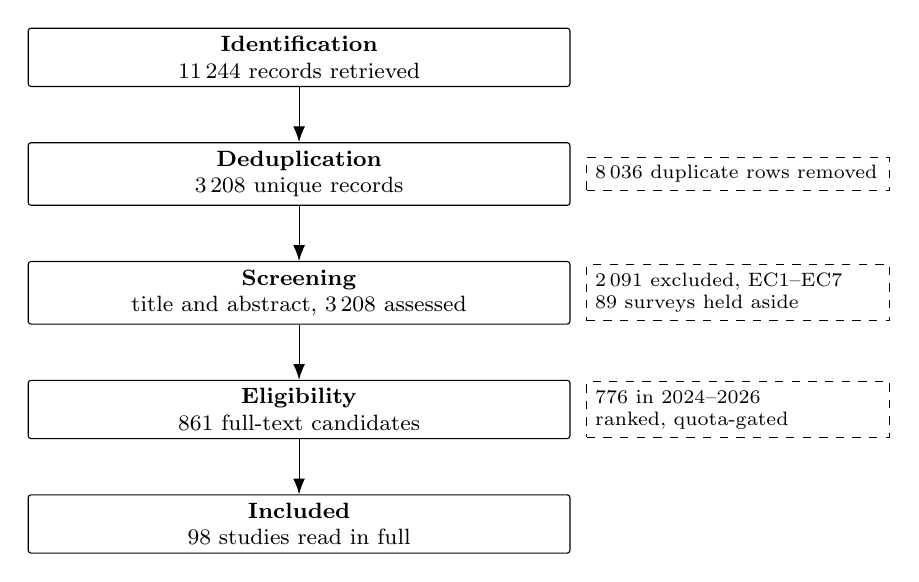
\begin{tikzpicture}[
      node distance=7mm,
      box/.style={draw, rounded corners=1pt, align=center, inner sep=3pt,
                  font=\footnotesize, text width=0.55\columnwidth},
      note/.style={draw, dashed, align=left, inner sep=3pt,
                   font=\scriptsize, text width=0.30\columnwidth},
      ar/.style={-{Latex[length=2mm]}}]
    \node[box] (id) {\textbf{Identification}\\ \CorpusRaw{} records retrieved};
    \node[box, below=of id] (dd) {\textbf{Deduplication}\\ \CorpusDedup{} unique records};
    \node[box, below=of dd] (sc) {\textbf{Screening}\\ title and abstract, \CorpusDedup{} assessed};
    \node[box, below=of sc] (el) {\textbf{Eligibility}\\ \ScrInclude{} full-text candidates};
    \node[box, below=of el] (in) {\textbf{Included}\\ \ReadTotal{} studies read in full};
    \draw[ar] (id) -- (dd); \draw[ar] (dd) -- (sc);
    \draw[ar] (sc) -- (el); \draw[ar] (el) -- (in);
    \node[note, right=2mm of dd.east, anchor=west]
      {\CorpusDupes{} duplicate rows removed};
    \node[note, right=2mm of sc.east, anchor=west]
      {\ScrExclude{} excluded, EC1--EC7\\ \ScrSurvey{} surveys held aside};
    \node[note, right=2mm of el.east, anchor=west]
      {\ReadPool{} in \ReadFrom--\ReadTo{}\\ ranked, quota-gated};
  \end{tikzpicture}
  \caption{PRISMA flow. Counts are generated from the harvest log
  (retrieved \HarvestDate{}); the window is \HarvestWindow{}.
  Fig.~\ref{fig:selection} expands the identification and selection stages.}
  \label{fig:prisma}
\end{figure}

\begin{figure*}[!t]
  \centering
  % Generated by tools/make_flow_diagram.py from the harvest logs.
  \resizebox{\textwidth}{!}{% Generated by tools/make_flow_diagram.py -- do not edit by hand.
% Every count is read from data/*.json at build time.
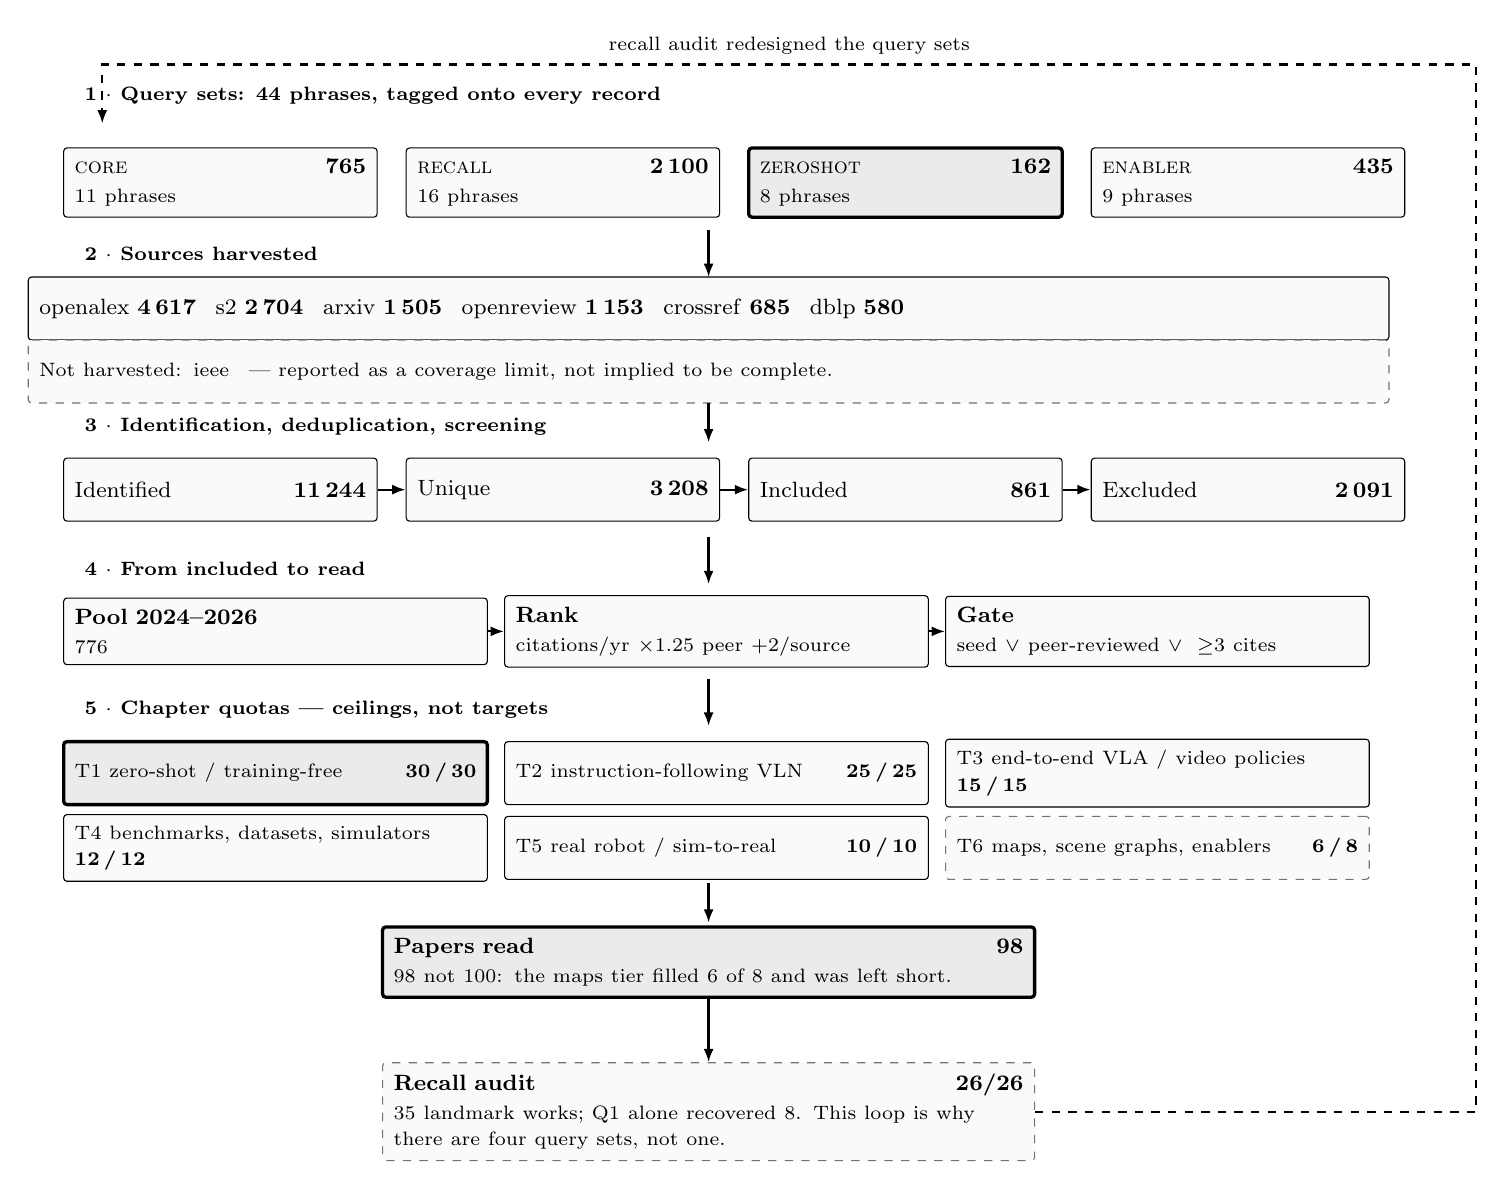
\begin{tikzpicture}[
    font=\footnotesize,
    bx/.style={draw, rounded corners=1.2pt, align=left, inner sep=4pt,
               minimum height=8mm, fill=black!2},
    hi/.style={bx, fill=black!8, very thick},
    wr/.style={bx, draw=black!55, dashed},
    bandlab/.style={font=\scriptsize\bfseries, anchor=west},
    ar/.style={-{Latex[length=1.7mm]}, thick},
    fb/.style={-{Latex[length=1.7mm]}, thick, dashed}]

\node[bandlab] at (0,0.55) {1 $\cdot$ Query sets: 44 phrases, tagged onto every record};
\node[bx, text width=3.7cm] (q0) at (1.85,-0.55) {\textsc{core}\hfill\textbf{765}\\[1pt]\scriptsize 11 phrases};
\node[bx, text width=3.7cm] (q1) at (6.20,-0.55) {\textsc{recall}\hfill\textbf{2\,100}\\[1pt]\scriptsize 16 phrases};
\node[hi, text width=3.7cm] (q2) at (10.55,-0.55) {\textsc{zeroshot}\hfill\textbf{162}\\[1pt]\scriptsize 8 phrases};
\node[bx, text width=3.7cm] (q3) at (14.90,-0.55) {\textsc{enabler}\hfill\textbf{435}\\[1pt]\scriptsize 9 phrases};
\draw[ar] (8.05,-1.15) -- (8.05,-1.75);
\node[bandlab] at (0,-1.45) {2 $\cdot$ Sources harvested};
\node[bx, text width=17.0cm] (src) at (8.05,-2.15) {openalex~\textbf{4\,617} \, s2~\textbf{2\,704} \, arxiv~\textbf{1\,505} \, openreview~\textbf{1\,153} \, crossref~\textbf{685} \, dblp~\textbf{580}};
\node[wr, text width=17.0cm] (nosrc) at (8.05,-2.95) {\scriptsize Not harvested: ieee \, --- reported as a coverage limit, not implied to be complete.};
\draw[ar] (8.05,-3.35) -- (8.05,-3.85);
\node[bandlab] at (0,-3.65) {3 $\cdot$ Identification, deduplication, screening};
\node[bx, text width=3.7cm] (s0) at (1.85,-4.45) {Identified\hfill\textbf{11\,244}};
\node[bx, text width=3.7cm] (s1) at (6.20,-4.45) {Unique\hfill\textbf{3\,208}};
\draw[ar] (s0) -- (s1);
\node[bx, text width=3.7cm] (s2) at (10.55,-4.45) {Included\hfill\textbf{861}};
\draw[ar] (s1) -- (s2);
\node[bx, text width=3.7cm] (s3) at (14.90,-4.45) {Excluded\hfill\textbf{2\,091}};
\draw[ar] (s2) -- (s3);
\draw[ar] (8.05,-5.05) -- (8.05,-5.65);
\node[bandlab] at (0,-5.45) {4 $\cdot$ From included to read};
\node[bx, text width=5.1cm] (r0) at (2.55,-6.25) {\textbf{Pool 2024--2026}\\[1pt]\scriptsize 776};
\node[bx, text width=5.1cm] (r1) at (8.15,-6.25) {\textbf{Rank}\\[1pt]\scriptsize citations/yr $\times$1.25 peer $+$2/source};
\draw[ar] (r0) -- (r1);
\node[bx, text width=5.1cm] (r2) at (13.75,-6.25) {\textbf{Gate}\\[1pt]\scriptsize seed $\vee$ peer-reviewed $\vee\ \geq$3 cites};
\draw[ar] (r1) -- (r2);
\draw[ar] (8.05,-6.85) -- (8.05,-7.45);
\node[bandlab] at (0,-7.25) {5 $\cdot$ Chapter quotas --- ceilings, not targets};
\node[hi, text width=5.1cm] at (2.55,-8.05) {\scriptsize T1 zero-shot / training-free\hfill\textbf{30\,/\,30}};
\node[bx, text width=5.1cm] at (8.15,-8.05) {\scriptsize T2 instruction-following VLN\hfill\textbf{25\,/\,25}};
\node[bx, text width=5.1cm] at (13.75,-8.05) {\scriptsize T3 end-to-end VLA / video policies\hfill\textbf{15\,/\,15}};
\node[bx, text width=5.1cm] at (2.55,-9.00) {\scriptsize T4 benchmarks, datasets, simulators\hfill\textbf{12\,/\,12}};
\node[bx, text width=5.1cm] at (8.15,-9.00) {\scriptsize T5 real robot / sim-to-real\hfill\textbf{10\,/\,10}};
\node[wr, text width=5.1cm] at (13.75,-9.00) {\scriptsize T6 maps, scene graphs, enablers\hfill\textbf{6\,/\,8}};
\draw[ar] (8.05,-9.45) -- (8.05,-9.95);
\node[hi, text width=8.0cm] (read) at (8.05,-10.45) {\textbf{Papers read}\hfill\textbf{98}\\[1pt]\scriptsize 98 not 100: the maps tier filled 6 of 8 and was left short.};
\node[wr, text width=8.0cm] (aud) at (8.05,-12.35) {\textbf{Recall audit}\hfill\textbf{26/26}\\[1pt]\scriptsize 35 landmark works; Q1 alone recovered 8. This loop is why there are four query sets, not one.};
\draw[ar] (read) -- (aud);
\draw[fb] (aud.east) -- (17.8,-12.35) -- (17.8,0.95) -- (0.35,0.95)
     node[midway, above, font=\scriptsize] {recall audit redesigned the query sets} -- (0.35,0.2);
\end{tikzpicture}
}
  \caption{How the \ReadTotal{} studies were found and chosen. Left to
  right: the four query sets and their unique yields, the six harvested
  sources, identification and screening, the ranking of the
  \ReadFrom--\ReadTo{} pool, and the per-chapter quotas. The dashed return
  path is the recall audit of Sec.~\ref{sec:validation}, which is what
  caused the query set to be redesigned. Every number in the figure is read
  from the harvest log at build time.}
  \label{fig:selection}
\end{figure*}

\subsection{From the Included Set to the Papers Read}\label{sec:readinglist}
\ScrInclude{} included records is more than can be read closely, so the
selection to \ReadTotal{} is stated explicitly rather than left to
judgement. The pool was first restricted to \ReadFrom--\ReadTo{},
leaving \ReadPool{} records, on the grounds that the earlier included work
is covered adequately as background. Each record was then scored by
citations per year since publication --- which prevents 2023 papers from
dominating 2026 ones on raw counts --- multiplied by 1.25 if peer-reviewed,
plus two points for each independent source that returned it, plus a large
constant for the hand-curated seed works so that they are pinned in
regardless of citation count. A record was eligible only if it was a seed,
was peer-reviewed, or had at least three citations.

Ranked records were then drawn into six chapter quotas: zero-shot and
training-free (30\%), instruction-following VLN (25\%), end-to-end VLA and
video policies (15\%), benchmarks and simulators (12\%), real-robot and
sim-to-real (10\%), and mapping and enabling representations (8\%). The
quotas are ceilings, not targets: the mapping tier filled only 6 of its 8
places because too few in-window records met the eligibility bar, and the
shortfall was left rather than backfilled with weaker papers. This is why
the reading set is \ReadTotal{} and not 100.

\subsection{Snowballing}
Backward snowballing was performed from the reference lists of the
\ReadTotal{} read papers; forward snowballing used the Semantic Scholar
cited-by graph restricted to the window. Both were seeded from five entry
points spanning the taxonomy: VLFM~\cite{yokoyama2024vlfm} for frontier
methods, NaVid~\cite{zhang2024navid} for video VLAs,
ETPNav~\cite{an2025etpnav} for continuous VLN,
HOV-SG~\cite{werby2024hierarchical} for open-vocabulary mapping, and
GOAT-Bench~\cite{khanna2024goat} for benchmarks.

\subsection{Search Validation}\label{sec:validation}
A hand-curated set of \SeedTotal{} landmark works serves as a recall check:
after every change to the query set, the corpus is tested for how many of
them it returns. The final configuration recovers \RecallWindow{} of the
seed works published inside the window; the remainder are pre-2023 and
excluded by IC1.

The interesting result is the failure that preceded it. A single canonical
query --- the phrase family a reviewer would expect, run against Scopus in
the conventional way --- recovers only 8 of \SeedTotal{} seeds. The misses
fall into three groups, and each one implies a change to the protocol.
Works filed under a different task name (ObjectNav, embodied navigation,
semantic navigation) are invisible to a query built from
``vision-and-language navigation'' and its hyphenation variants. Works whose
contribution is a representation rather than a policy ---
VLMaps, ConceptFusion~\cite{jatavallabhula2023conceptfusion},
ConceptGraphs~\cite{gu2023conceptgraphs}, Code as
Policies~\cite{liang2022code} --- never use ``navigation'' in the title at
all, yet the zero-shot systems in Sec.~\ref{sec:zeroshot} are built
directly on them. And works at NeurIPS, ICLR and CoRL are absent from the
conventional indexes irrespective of the query.

The four consequences were: add the \textsc{recall} set for adjacent task
names; add the \textsc{enabler} set for representation papers; add
OpenReview as a first-class source; and treat Semantic Scholar rather than
OpenAlex as the citation authority. We report this because it is
generalisable: any systematic review of this literature that runs one
canonical query against one conventional index will miss roughly
three-quarters of its own landmark works, and will do so silently.

\subsection{Threats to Validity}\label{sec:threats}
\emph{Coverage.} IEEE Xplore was not harvested. Given the overlap between
IEEE conference proceedings and the DBLP, Crossref and OpenAlex records we
did harvest, we expect the marginal loss to be small but we cannot bound
it. \FailedRequests{} requests exhausted their retry budget under rate
limiting; the affected pages are logged, and their true counts are unknown
rather than assumed to be zero.

\emph{Screening reliability.} Screening was performed by a single author,
which risks systematic bias no resample can detect. The automated
pre-screen applies the same phrase-level rules to every arm of the
taxonomy, so it cannot preferentially favour zero-shot or supervised work,
but the adjudication of the \ScrCheck{} flagged records was manual.

\emph{Currency versus reliability.} Including preprints keeps the survey
current at the cost of admitting unrefereed claims. This bites hardest in
the VLA tier, where only 6 of 15 selected papers are peer-reviewed. We mark
supervision and venue type in every comparison table so that a reader can
discount preprint-only results.

\emph{Citation signal.} Roughly half of the deduplicated corpus carries a
2026 date, where citation counts have had almost no time to accumulate. The
per-year normalisation reduces but does not remove the resulting noise, and
recent work is therefore selected substantially on venue and seed status
rather than on impact.
% =====================================================================
\section{Taxonomy}\label{sec:taxonomy}
Surveys of this literature usually branch on the task (R2R, ObjectNav,
dialogue) or on the backbone family (transformer, LLM, VLA). Both choices
scatter systems that solve the same problem into different chapters. We
branch instead on the \emph{architectural role the foundation model plays},
which is the decision that determines what data a system needs, what it can
generalise over, and what it costs per step. Supervision level is then an
orthogonal attribute --- a shading in Fig.~\ref{fig:taxonomy}, a column in
Table~\ref{tab:methods} --- rather than a branch, precisely so that a
training-free and a fully trained solution to the same problem sit next to
each other.

\subsection{R1: The Model as External Reasoner}
The navigation policy is a prompt. Observations are converted into text or
into a scored spatial structure, a frozen LLM or VLM selects the next
subgoal, and a classical planner executes it. No gradient touches a
navigation objective. Siblings are separated by \emph{what the model is
shown}: a verbalised panorama~\cite{long2024discuss,qiao2025open}, a
running linguistic map~\cite{chen2024mapgpt}, a top-view
projection~\cite{zhong2026topv,zhang2025mapnav}, a 3D scene
graph~\cite{yin2024online,werby2024hierarchical,yin2025unigoal}, or a
frontier-scored value map~\cite{yokoyama2024vlfm,nie2025wmnav,long2024instructnav}.
Sec.~\ref{sec:zeroshot} treats this branch in detail.

\subsection{R2: The Model as Perception Backbone}
A frozen encoder supplies features or detections, and a separately trained
policy consumes them. The foundation model contributes open-vocabulary
recognition but not decision-making. This is the quiet majority of the
field: waypoint predictors, semantic mappers and value heads are trained on
navigation data while CLIP, Grounding DINO or SAM remain frozen. The
branch matters because it is the source of most disputed zero-shot claims
--- a system with a frozen VLM and a trained waypoint predictor is
training-free in one component and supervised in another.

\subsection{R3: The Model as the Policy}
A multimodal LLM is fine-tuned to emit actions directly, taking video or
frame sequences as input and low-level or mid-level commands as output.
NaVid~\cite{zhang2024navid} established the video-VLM formulation;
Uni-NaVid~\cite{zhang2024navidb} unified several embodied tasks in one
model; NaVILA~\cite{cheng2024navila} split the stack into a VLA level and a
learned locomotion level; StreamVLN~\cite{wei2025streamvln} made the
formulation streaming and cache-efficient. Siblings are separated by the
action interface and by whether the visual memory is explicit or implicit.

\subsection{R4: The Model as Data Engine}
The foundation model never runs at test time. It generates instructions,
trajectories or scenes offline, and a conventional policy is trained on the
result. RoomTour3D~\cite{han2025roomtour} derives instruction data from real
room-tour video; OpenFly~\cite{gao2026openfly} synthesises aerial
trajectories at scale; SimWorld Studio~\cite{kang2026simworld} generates
environments. This branch is how zero-shot capability is converted into
supervised capability, and Sec.~\ref{sec:middle} argues it is the dominant
mechanism by which the field is currently advancing.

\subsection{R5: The Model as Critic or Selector}
The model neither perceives nor acts but judges: scoring candidate plans,
estimating uncertainty, or deciding when a more expensive module should be
invoked. VAMOS~\cite{castro2025vamos} rejects infeasible plans;
SURF~\cite{shinnick2026surf} reasons about when to invoke the expensive
model at all; Hydra-Nav~\cite{wang2026hydra} switches between a fast
reactive and a slow deliberative process. This is the newest branch and,
as Sec.~\ref{sec:eval} argues, the one most directly responsive to the
cost problem.

\begin{figure*}[!t]
  \centering
  % \includegraphics[width=\textwidth]{fig/taxonomy.pdf}
  \caption{Taxonomy of foundation-model navigation methods, branching on the
  role the model plays (R1--R5). Shading encodes supervision level, which is
  orthogonal to the role axis: a single role contains training-free,
  partially trained and fully supervised instances.}
  \label{fig:taxonomy}
\end{figure*}

% =====================================================================
\section{Environments, Datasets and Simulators}\label{sec:data}

\subsection{Photorealistic Scene Datasets}
Matterport3D~\cite{chang2017matterport3d} remains the substrate of the
discrete VLN benchmarks; HM3D~\cite{ramakrishnan2021habitat} supplies the
larger scene set that object-goal work has standardised on; HSSD and Gibson
appear as third and fourth evaluation domains in the stronger zero-shot
papers~\cite{wu2024voronav,zhou2025beliefmapnav}. Scanned scenes carry a
structural limitation that the field has begun to confront: reconstruction
artefacts, missing ceilings and floor-level noise are not the failure modes
a real robot encounters, so success on them is a necessary but weak
condition for deployment.

\subsection{Simulators}
Habitat~\cite{savva2019habitat} dominates, with AI2-THOR~\cite{kolve2017ai2} and its procedural
extension ProcTHOR~\cite{deitke2022procthor} supplying the interactive
alternative. Two developments in the window matter more than incremental
speed. First, VLN-PE~\cite{wang2025rethinking} instantiates VLN across
humanoid, quadruped and wheeled platforms inside a physics simulator,
turning ``embodiment'' from an assumption into an experimental variable.
Second, aerial platforms acquired dedicated
infrastructure: OpenUAV~\cite{wang2025towards} provides realistic UAV flight
dynamics for VLN, and OpenFly~\cite{gao2026openfly} a full aerial platform
and dataset.

\subsection{Instruction Corpora and Their Generation}
The window contains a clear phase change in how instruction data is
obtained. R2R-CE provides 5.6K English trajectories and RxR-CE 126K
multilingual instructions across English, Hindi and
Telugu~\cite{wei2025streamvln}, all human-annotated. Against this,
the training sets assembled during the window are one to three orders of
magnitude larger and almost entirely machine-generated:
NaVid~\cite{zhang2024navid} trains on 510K navigation samples plus 763K
auxiliary samples; Uni-NaVid~\cite{zhang2024navidb} on 3.6M;
NavFoM~\cite{zhang2025embodied} on 8M navigation samples spanning
embodiments and camera configurations; ABot-N0~\cite{chu2026abot} reports
16.9M trajectories. CityNav~\cite{lee2024citynav} is the notable
counter-example, contributing 32{,}637 \emph{real} human demonstrations for
aerial city-scale navigation.

This shift has an evaluation consequence that Sec.~\ref{sec:eval} returns
to. When training instructions are generated by a language model, and
evaluation instructions are drawn from the same generator family, the
benchmark measures agreement with the generator rather than with human
language use.

\subsection{Data Augmentation and Synthetic Environments}
Three strategies appear. Instruction augmentation generates new language for
existing trajectories. Trajectory augmentation samples new paths through
existing scenes, which is how the largest corpora above are built. Scene
augmentation generates the environments themselves;
SimWorld Studio~\cite{kang2026simworld} automates environment generation,
and RoomTour3D~\cite{han2025roomtour} takes the opposite route of mining
real video tours for geometry-aware instruction data. The open question,
stated in Sec.~\ref{sec:challenges}, is whether policies trained
predominantly on generated data inherit the generator's blind spots.

\subsection{Benchmarks Targeting Generalisation}
Four benchmarks in the window are explicitly designed to break agents
rather than rank them. HM3D-OVON~\cite{yokoyama2024ovon} raises the
object-goal vocabulary to 379 categories, which invalidates any method
that quietly assumes a closed label set. GOAT-Bench~\cite{khanna2024goat}
mixes category, language and image goals within a single lifelong episode
sequence, so an agent cannot specialise to one goal modality.
UAV-ON~\cite{xiao2025benchmark} moves open-world object-goal navigation
into the air. NavBench~\cite{qiao2025navbench} and
NaviTrace~\cite{windecker2025navitrace} probe multimodal LLMs directly and
score them against human trajectories, separating navigational competence
from the ability to produce plausible navigation text ---
a distinction Sec.~\ref{sec:eval} argues the standard metrics cannot make.

\begin{table*}[!t]
  \caption{Environments, datasets and benchmarks in the reviewed window.
  Scale figures are as reported by the cited work; ``real'' distinguishes
  human-collected trajectories from machine-generated ones.}
  \label{tab:datasets}
  \centering
  \setlength{\tabcolsep}{3pt}
  \footnotesize
  \begin{tabular}{llllll}
    \toprule
    Resource & Type & Domain & Goal modality & Scale as reported & Role in this survey \\
    \midrule
    Matterport3D~\cite{chang2017matterport3d} & Scene dataset & Indoor & --- & Scanned buildings & Substrate of R2R/RxR/REVERIE \\
    HM3D~\cite{ramakrishnan2021habitat}       & Scene dataset & Indoor & --- & Large scene set & Standard ObjectNav domain \\
    AI2-THOR~\cite{kolve2017ai2}              & Simulator     & Indoor & --- & Interactive & Interactive alternative to Habitat \\
    ProcTHOR~\cite{deitke2022procthor}        & Generator     & Indoor & --- & Procedural & Scale for on-policy RL~\cite{zeng2024poliformer} \\
    \midrule
    R2R-CE~\cite{krantz2020beyond}            & Benchmark & Indoor & Step-by-step route & 5.6K English traj.~\cite{wei2025streamvln} & Primary continuous VLN benchmark \\
    RxR-CE~\cite{ku2020room}                  & Benchmark & Indoor & Step-by-step, 3 languages & 126K instructions~\cite{wei2025streamvln} & Long-horizon, multilingual \\
    REVERIE~\cite{qi2019reverie}              & Benchmark & Indoor & Object + coarse hint & --- & Remote object grounding \\
    SOON~\cite{zhu2021soon}                   & Benchmark & Indoor & Scenario description & --- & Coarse goal specification \\
    CVDN~\cite{thomason2019vision}            & Benchmark & Indoor & Dialogue history & --- & Under-specified goals \\
    \midrule
    HM3D-OVON~\cite{yokoyama2024ovon}         & Benchmark & Indoor & Open-vocabulary category & 379 categories & Breaks closed label sets \\
    GOAT-Bench~\cite{khanna2024goat}          & Benchmark & Indoor & Category / language / image & Lifelong sequences & Multi-modal, lifelong \\
    UAV-ON~\cite{xiao2025benchmark}           & Benchmark & Aerial & Open-world object goal & --- & Aerial generalisation \\
    NavBench~\cite{qiao2025navbench}          & Probe     & Indoor & --- & --- & Probes MLLM navigational ability \\
    NaviTrace~\cite{windecker2025navitrace}   & Probe     & Mixed  & Language & Human-referenced & Human-gap measurement \\
    VLN-PE~\cite{wang2025rethinking}          & Platform  & Indoor & Step-by-step route & Humanoid/quadruped/wheeled & Embodiment as a variable \\
    \midrule
    OpenFly~\cite{gao2026openfly}             & Platform + data & Aerial & Step-by-step route & 100K trajectories & Aerial VLN at scale \\
    OpenUAV~\cite{wang2025towards}            & Platform  & Aerial & Step-by-step route & --- & Realistic UAV dynamics \\
    CityNav~\cite{lee2024citynav}             & Dataset   & Aerial/urban & Language goal & 32{,}637 real traj. & Real human demonstrations \\
    RoomTour3D~\cite{han2025roomtour}         & Dataset   & Indoor & Generated instructions & From real tour video & Geometry-aware video tuning \\
    SimWorld Studio~\cite{kang2026simworld}   & Generator & Urban & --- & Automatic & Environment synthesis \\
    \bottomrule
  \end{tabular}
\end{table*}
% =====================================================================
\section{Visual Perception and Scene Representation}\label{sec:perception}
Across the corpus, the single design choice that best predicts what a
navigation agent can and cannot do is not its backbone but its spatial
representation. This section catalogues the options; Sec.~\ref{sec:zeroshot}
shows that the progression of zero-shot performance during the window is
almost exactly a progression through this list.

\subsection{Frame-Level Encoders}
Contrastive image--text encoders~\cite{radford2021learning} provide the
scoring function that makes an open-vocabulary goal meaningful, and remain
the default. Captioning and instruction-tuned
VLMs~\cite{li2023blip,liu2023visual} are used where a textual description
rather than a similarity score is required --- VLFM~\cite{yokoyama2024vlfm}
uses BLIP-2 to produce the value that drives its frontier map. Open-set
detection~\cite{liu2023grounding} and promptable
segmentation~\cite{kirillov2023segment} supply localisation; AO-Planner's
affordance-grounded waypoints~\cite{chen2024affordances} are built on the
latter.

\subsection{Panoramic versus Monocular Observation}
The panoramic assumption inherited from R2R is convenient and unphysical.
It supplies, at every step, a complete view of the local surroundings that a
forward-facing robot camera does not have. Systems designed for deployment
are consequently monocular: NaVid~\cite{zhang2024navid} takes a monocular
video stream, and NavFoM~\cite{zhang2025embodied} reports the size of the
difference directly, with success falling from 64.4\% in a multi-camera
configuration to 57.4\% with a single camera on VLN-CE RxR. Any comparison
that places panoramic and monocular agents in the same table without marking
the distinction is misleading, and Table~\ref{tab:methods} therefore carries
an observation column.

\subsection{Depth, Point Clouds and Geometry}
Depth is what converts recognition into navigation, because it is what
allows a semantic observation to be projected into a map and hence into a
goal a planner can reach. The window contains a clear move towards richer
geometry: volumetric environment
representations~\cite{liu2024volumetric}, neural radiance
representations used for lookahead
prediction~\cite{wang2024lookahead}, and 3D feature fields used explicitly
as the sim-to-real bridge~\cite{wang2024real}.
JanusVLN~\cite{zeng2025janusvln} makes the geometric channel a first-class
component, maintaining separate implicit memories for semantics and
spatiality; ablating the spatial memory drops SPL from 49.2 to 40.9, which
is a large effect for a component that is often folded into a single
feature stream.

\subsection{Map Representations}
Five families appear, in rough order of increasing structure. \emph{Metric
semantic maps} project detections into a 2D grid. \emph{Value maps} score
each cell or frontier by its relevance to the
goal~\cite{yokoyama2024vlfm,long2024instructnav,chen2025constraint}.
\emph{Topological graphs} store viewpoints and their
connectivity~\cite{an2025etpnav,liu2025toponav}, which is what makes
backtracking expressible. \emph{Sparse geometric abstractions} such as the
Voronoi graph~\cite{wu2024voronav} reduce the map to a decision skeleton
that fits in a prompt. \emph{Volumetric belief representations} carry
uncertainty explicitly; BeliefMapNav~\cite{zhou2025beliefmapnav} maintains a
3D voxel belief map and reports that removing the posterior update costs
10.4\% success, while relying on spatial priors alone costs 8.5\%.

Modular 3D scene representations for cognitive
planning~\cite{s2024cognitive} and language-driven strategies that fuse a
semantic map with an LLM prior~\cite{zhong2024language} occupy the middle of
this range, trading representational richness for tractability.

A distinct and pragmatic branch renders the map \emph{back into an image}
for a multimodal model to read. MapNav~\cite{zhang2025mapnav} annotates a
semantic map for this purpose and TopV-Nav~\cite{zhong2026topv} reasons
directly in the top view. The motivation is that current MLLMs are much
better at reading a picture of a map than at integrating a sequence of
egocentric frames into one.

\subsection{Open-Vocabulary and Language-Queryable Maps}\label{sec:ovmaps}
This is the structural enabler of the entire zero-shot branch, and it
originates outside navigation. Visual language maps~\cite{huang2022visual}, open-vocabulary queryable
scene representations~\cite{chen2022open}, open-set multimodal
mapping~\cite{jatavallabhula2023conceptfusion} and open-vocabulary 3D scene
graphs~\cite{gu2023conceptgraphs} make a map queryable by arbitrary text.
Once that exists, ``go to the cat-shaped mug'' becomes a map query rather
than a learning problem.

The navigation-specific development in the window is hierarchy and
online construction. HOV-SG~\cite{werby2024hierarchical} builds hierarchical
open-vocabulary 3D scene graphs spanning floors, rooms and objects, and
reports a 75\% reduction in representation size relative to dense
alternatives --- which is what makes multi-floor, building-scale operation
tractable. SG-Nav~\cite{yin2024online} constructs the scene graph
\emph{online} during the episode and prompts the LLM with it hierarchically.
UniGoal~\cite{yin2025unigoal} reformulates several goal types as graph
matching against such a representation, which is how one zero-shot system
covers object, instance and text goals without retraining.
VL-Nav~\cite{du2025neuro} carries the idea onto hardware.

\subsection{Memory}
Three mechanisms are in use. \emph{Explicit textual memory} accumulates a
running description --- MapGPT's online linguistic map~\cite{chen2024mapgpt}
is the clearest instance, and its appeal is that it is directly readable by
the planner. \emph{Structured memory} keeps a graph or map, which supports
revisiting and backtracking but must be maintained.
\emph{Implicit memory} keeps model state: StreamVLN~\cite{wei2025streamvln}
uses a SlowFast context with KV-cache reuse and voxel-based spatial pruning,
cutting visual tokens by roughly 30\% with only slight performance loss,
and JanusVLN's dual memory~\cite{zeng2025janusvln} is implicit by
construction. NavMorph~\cite{yao2025navmorph} extends memory into a
self-evolving world model that adapts within the test episode.

% =====================================================================
\section{Language Understanding and Cross-Modal Grounding}\label{sec:language}

\subsection{Instruction Decomposition}
Long instructions are not executed as units. Every competitive system in the
corpus decomposes them, and the differences lie in when and how the
decomposition is revised. InstructNav's Dynamic Chain-of-Navigation
unifies decomposition across instruction types, which is what lets one
system address route-following, object goals and demand-driven goals
without task-specific machinery~\cite{long2024instructnav}. CA-Nav's
constraint-aware sub-instruction manager decomposes the instruction into
sub-instructions with explicit completion
constraints and switches only when those constraints are
satisfied~\cite{chen2025constraint}; because switching is
constraint-triggered rather than per-step, the LLM need not be called at
every decision, which is the source of its cost advantage.
NavCoT~\cite{lin2025navcot} instead trains the decomposition, using
parameter-efficient in-domain tuning to elicit navigational chain-of-thought
from a small model.

\subsection{Cross-Modal Attention and Alignment}
The supervised lineage --- recurrent cross-modal
BERT~\cite{hong2020vln}, history-aware
transformers~\cite{chen2021history}, dual-scale graph
transformers~\cite{chen2022think} --- established the alignment machinery
that later systems inherit. The window's contribution to it is causal
rather than architectural: GOAT~\cite{wang2024vision} attacks the spurious
correlations that cross-modal attention learns, with backdoor and frontdoor
adjustment losses that target dataset bias directly. This matters for
generalisation claims, since an agent that has learned the layout statistics
of Matterport3D rather than the language--percept correspondence will fail
in exactly the settings the field cares about.

\subsection{Open-Vocabulary Grounding}
Grounding an arbitrary noun phrase is the capability that separates the
window from what preceded it, and it is where the honest limits show. The
``cat-shaped mug'' formulation~\cite{dorbala2024embodied} names the problem
precisely: the goal is a compositional description, not a category, and no
label set contains it. Prioritized Semantic
Learning~\cite{sun2024prioritized} addresses the instance-level case, where
the agent must distinguish one instance of a category from another.
Grounding quality is also the ceiling on the whole R1 branch --- when the
detector does not fire on the target, no amount of LLM reasoning recovers
the episode, a failure mode Sec.~\ref{sec:zsfail} returns to.

\subsection{Spatial and Relational Language}
Instructions are dense in spatial relations, and this is the weakest link in
current multimodal models. Several papers in the corpus exist specifically
to work around it. TopV-Nav~\cite{zhong2026topv} argues that MLLMs reason
better in a top view than over egocentric sequences and reports gains of
6.5\% SR and 2.2\% SPL on MP3D from doing so.
Spatial-representation work for aerial
navigation~\cite{gao2026exploring} and reachability-aware spatial
grounding~\cite{zhang2026what} make similar structural concessions.
NavBench~\cite{qiao2025navbench} probes the underlying ability directly
rather than through task success, and it is the appropriate reference for
the claim that spatial reasoning, not language understanding, is the
bottleneck.

\subsection{Dialogue and Ambiguous Instructions}
Real instructions are under-specified. CVDN~\cite{thomason2019vision}
formalises the dialogue setting; within the window the emphasis moves to
quantifying ambiguity rather than resolving it by asking.
Guo~\emph{et al.}~\cite{guo2026quantifying} quantify the uncertainty that
instruction ambiguity induces in a VLN agent, and
SURF~\cite{shinnick2026surf} makes selective uncertainty reasoning the
trigger for expensive computation. DiscussNav~\cite{long2024discuss} takes
the multi-agent route, assigning distinct expert roles to separate model
invocations and having them discuss before the agent moves.

% =====================================================================
\section{Learned Navigation Policies}\label{sec:policies}
Each subsection below follows the same template: the idea, representative
works, the training signal, and the failure mode that follows from it.

\subsection{Pre-Foundation Baselines}
Sequence-to-sequence and recurrent cross-modal
agents~\cite{hong2020vln}, history-aware
transformers~\cite{chen2021history} and topological graph
policies~\cite{chen2022think} define the pre-window state of the art.
They are trained on human demonstrations with imitation and auxiliary
losses. Their failure mode is the one that motivates the whole survey: they
do not transfer to instructions or goals outside the annotated
distribution.

\subsection{Vision-Language Pretraining Agents}
The bridging generation keeps the trained policy but replaces hand-designed
features with pretrained multimodal representations.
ETPNav~\cite{an2025etpnav} is the strongest representative and remains a
reference point for continuous VLN: it constructs a topological map online
and plans over it, reporting 57.21 SR and 49.15 SPL on the R2R-CE val-unseen
split, with gains of roughly 26 SR over recurrent-BERT baselines.
NavGPT-2~\cite{zhou2024navgpt} occupies the hinge position, recovering the
interpretability of LLM reasoning inside a trained VLN policy.

\subsection{MLLMs and VLMs Fine-Tuned as Policies}
This is the dominant paradigm of 2025--2026. The policy \emph{is} a
multimodal LLM, fine-tuned on navigation data.
NaVid~\cite{zhang2024navid} established the video formulation with a
monocular stream and no map, odometry or depth.
Uni-NaVid~\cite{zhang2024navidb} unified VLN, object navigation, embodied
question answering and human following in one video-VLA at 3.6M samples.
StreamVLN~\cite{wei2025streamvln} made it streaming, reaching 56.9\% SR and
51.9\% SPL on R2R-CE val-unseen and 52.9\% SR / 46.0\% SPL on RxR-CE ---
comparable to ETPNav despite using RGB only, with no panoramic or waypoint
supervision. JanusVLN~\cite{zeng2025janusvln} adds explicit spatial memory.
Qwen-VLA~\cite{wang2026qwen} reports 69.0\% OSR on R2R and 59.6\% SR on RxR
while also covering manipulation benchmarks, and
NavFoM~\cite{zhang2025embodied} pushes the same idea to 8M samples across
embodiments and camera configurations.

Three variants extend the formulation past the indoor benchmark setting.
NaviLLM~\cite{zheng2024towards} introduces schema-based task specification to
train one generalist across embodied tasks, reporting a 29\% improvement on
CVDN. LeLaN~\cite{hirose2024lelan} learns a language-conditioned policy from
130 hours of unlabelled in-the-wild video, which is the corpus's clearest
attempt to escape simulator-derived training data altogether, and
OmniVLA~\cite{hirose2025omnivla} generalises it to an omni-modal goal
specification. EchoVLA~\cite{lin2025echovla} couples navigation and
manipulation in a single action model.

The training signal is behaviour cloning on generated trajectories, and the
failure mode follows from it: these systems inherit whatever the trajectory
generator could produce, and their open-vocabulary behaviour is bounded by
the diversity of the generated instruction set rather than by the backbone's
own vocabulary.

\subsection{Hierarchical and Modular Learned Systems}
Splitting the stack by time constant is the standard response to the cost
of running a large model in a control loop.
NaVILA~\cite{cheng2024navila} separates a VLA level emitting mid-level
language actions from a reinforcement-learned locomotion level that
executes them, which is what allows the same policy to drive a legged
robot. OmniNav~\cite{xue2025omninav} uses a fast--slow decomposition to hold
a 5\,Hz control rate. Hydra-Nav~\cite{wang2026hydra} makes the switch
adaptive and learned, invoking the slow deliberative process only at
stagnation points; it reduces the reasoning ratio to 3.0\% of steps while
reaching 72.9\% SR on HM3D, and improves on the best prior zero-shot system
by 12.1\% SR. VAMOS~\cite{castro2025vamos} places the hierarchy between
planning and feasibility, rejecting infeasible plans and reporting a
threefold improvement thereby.

\subsection{LLM-Augmented Training}
Here the foundation model shapes the training process and is then discarded.
Distillation of an LLM prior into a flow model~\cite{li2025distilling},
AO-Planner's distillation of its foundation-model waypoint planner into a
learned predictor~\cite{chen2024affordances}, and
ImagineNav's learned view-imagination module~\cite{zhao2024imaginenav} all
follow the pattern. VLD~\cite{milikic2025visual} takes the reward side of the same idea,
deriving a visual-language goal distance that can serve as a dense
reinforcement-learning signal where none is otherwise available.
Reinforcement learning has re-entered the field through
the same door: VLN-R1~\cite{qi2025vision} applies group-relative policy
optimisation with a time-decayed reward,
OctoNav~\cite{gao2025octonav} couples thinking-before-action supervision
with a navigation-specific GRPO variant, and
FlightGPT~\cite{cai2025flightgpt} reports a 9.22\% improvement in the
aerial setting. PoliFormer~\cite{zeng2024poliformer} is the limiting case
--- pure on-policy RL with transformers at scale, reaching 85.5\% success
on CHORES-S without any LLM at inference time --- and it is the strongest
single piece of evidence that scale, not reasoning, may be the operative
variable.

\subsection{Uncertainty, Backtracking and Recovery}
An agent that cannot recognise it has gone wrong cannot recover.
SmartWay~\cite{shi2025smartway} adds backtracking to zero-shot continuous
VLN; E$^2$BA~\cite{shi2025environment} makes exploration and backtracking
the organising principle; SURF~\cite{shinnick2026surf} triggers on
uncertainty; NavMorph~\cite{yao2025navmorph} adapts its world model within
the episode. The presence of a distinct cluster of recovery-focused papers
in 2025--2026 is itself evidence that oscillation and commitment errors,
not perception, now dominate the residual failures in the strongest
systems.

\subsection{Comparative Summary}
Table~\ref{tab:methods} summarises representative systems. Two columns
carry most of the information. \emph{Observation} distinguishes panoramic
from monocular agents, without which the success figures are not
comparable. \emph{Supervision} states plainly what was trained, which is
the input to the zero-shot audit in Table~\ref{tab:zsaudit}.

\begin{table*}[!t]
  \caption{Representative methods. Figures are as reported by the cited
  paper on the stated split; they are \emph{not} normalised across papers,
  and Sec.~\ref{sec:comparability} explains why cross-row comparison is
  unsafe. Pan.\ = panoramic, Mono.\ = monocular.}
  \label{tab:methods}
  \centering
  \setlength{\tabcolsep}{3pt}
  \footnotesize
  \begin{tabular}{lllllll}
    \toprule
    Method & Role & Observation & Spatial representation & Supervision & Benchmark (split) & Reported \\
    \midrule
    \multicolumn{7}{l}{\itshape Training-free planners (R1)} \\
    VLFM~\cite{yokoyama2024vlfm}          & R1 & RGB-D  & 2D value map        & None (frozen VLM)      & ObjectNav HM3D & 52.5 SR / 30.4 SPL$^\dagger$ \\
    ESC~\cite{zhou2023esc}                & R1 & RGB-D  & Semantic map        & None                   & ObjectNav HM3D & 39.2 SR / 22.3 SPL$^\dagger$ \\
    L3MVN~\cite{yu2023l3mvn}              & R1 & RGB-D  & Semantic map        & None                   & ObjectNav HM3D & 50.4 SR / 23.1 SPL$^\dagger$ \\
    VoroNav~\cite{wu2024voronav}          & R1 & RGB-D  & Voronoi graph       & None                   & ObjectNav HM3D & 42.0 SR / 26.0 SPL$^\dagger$ \\
    OpenFMNav~\cite{kuang2024openfmnav}   & R1 & RGB-D  & Semantic map        & None                   & ObjectNav HM3D & 54.9 SR / 24.4 SPL$^\dagger$ \\
    TopV-Nav~\cite{zhong2026topv}         & R1 & RGB-D  & Top-view map        & None                   & ObjectNav HM3D & 45.9 SR / 28.0 SPL$^\dagger$ \\
    WMNav~\cite{nie2025wmnav}             & R1 & RGB-D  & Curiosity value map & None                   & ObjectNav HM3D & 58.1 SR / 31.2 SPL$^\dagger$ \\
    SG-Nav~\cite{yin2024online}           & R1 & RGB-D  & Online 3D scene graph & None                 & ObjectNav MP3D & $>$10\% SR over prior ZS \\
    InstructNav~\cite{long2024instructnav}& R1 & RGB-D  & Multi-source value maps & None & R2R-CE / ObjNav / DDN & first ZS R2R-CE \\
    CA-Nav~\cite{chen2025constraint}      & R1 & Mono.  & Constraint value map & None & R2R-CE / RxR-CE & +12/+13\% SR over ZS \\
    \midrule
    \multicolumn{7}{l}{\itshape Trained policies (R2, R3)} \\
    ETPNav~\cite{an2025etpnav}            & R2 & Pan.   & Topological graph   & Full VLN               & R2R-CE val-unseen & 57.21 SR / 49.15 SPL \\
    NaVid~\cite{zhang2024navid}           & R3 & Mono.  & None (implicit)     & 510K + 763K samples    & R2R-CE & video VLA baseline \\
    Uni-NaVid~\cite{zhang2024navidb}      & R3 & Mono.  & None (implicit)     & 3.6M samples           & VLN-CE R2R / RxR & +3.6 SR on RxR \\
    StreamVLN~\cite{wei2025streamvln}     & R3 & Mono.  & KV-cache memory & VLN + 150K ScaleVLN & R2R-CE / RxR-CE & 56.9/51.9; 52.9/46.0 \\
    JanusVLN~\cite{zeng2025janusvln}      & R3 & Mono.  & Dual implicit memory & VLN                   & RxR-CE & 40.8 $\to$ 44.9 SR \\
    NavFoM~\cite{zhang2025embodied}       & R3 & Multi  & None (implicit)     & 8M samples             & VLN-CE RxR & 57.4 (mono) / 64.4 (multi) SR \\
    Qwen-VLA~\cite{wang2026qwen}          & R3 & Mono.  & None (implicit)     & Multi-task             & R2R / RxR & 69.0 OSR / 59.6 SR \\
    PoliFormer~\cite{zeng2024poliformer}  & R2 & Mono.  & None (implicit)     & On-policy RL           & CHORES-S & 85.5 SR \\
    RoboTron-Nav~\cite{zhong2025robotron} & R3 & Mono.  & None (implicit)     & Multi-task             & CHORES-S & 72.1 SR / 53.0 SEL \\
    Hydra-Nav~\cite{wang2026hydra}        & R5 & Mono.  & Dual-process & IRFT & ObjectNav HM3D & 72.9 SR; 3.0\% reasoning \\
    \bottomrule
    \multicolumn{7}{l}{\footnotesize $^\dagger$ As tabulated by WMNav~\cite{nie2025wmnav}, Table~I --- one common source, so these rows \emph{are} mutually comparable.}
  \end{tabular}
\end{table*}
% =====================================================================
\section{Zero-Shot and Training-Free Navigation}\label{sec:zeroshot}
This is the chapter the survey exists for. We first show that ``zero-shot''
denotes at least five distinct claims, then audit what the surveyed systems
actually do, then trace the quantitative arc of the paradigm across the
window, and finally state what we take to be the honest conclusion: that
zero-shot navigation established the field's architecture and then lost
its numerical lead to trained models that had absorbed it.

\subsection{What ``Zero-Shot'' Means in VLN}\label{sec:zs-defs}
We distinguish five senses.

\begin{IEEEdescription}[\IEEEsetlabelwidth{ZS-5}]
\item[ZS-1] \emph{Training-free.} No gradient update is performed on any
navigation-specific objective. The policy is a frozen model plus a prompt.
\item[ZS-2] \emph{Open-vocabulary goal.} The goal may be any noun phrase;
it need not appear in any label set the system was built with.
\item[ZS-3] \emph{Cross-dataset.} The agent is trained on dataset A and
evaluated on dataset B without adaptation.
\item[ZS-4] \emph{Unseen environment.} The agent is evaluated on the
standard validation-unseen split of the dataset it was trained on.
\item[ZS-5] \emph{Cross-embodiment or sim-to-real.} The agent is deployed on
a morphology, sensor configuration or physical platform it never trained on.
\end{IEEEdescription}

Two observations follow immediately. First, ZS-4 is not zero-shot in any
useful sense --- it is the ordinary generalisation split that supervised VLN
has always reported --- yet several papers in the corpus present it as
though it were, and readers comparing a ZS-1 system against a ZS-4 system
are comparing incomparable things. Second, the senses are independent:
PSL~\cite{sun2024prioritized} is ZS-2 but not ZS-1, since it trains a policy
while avoiding object annotations; VLFM~\cite{yokoyama2024vlfm} is ZS-1 at
the semantic level while containing a low-level controller trained with
reinforcement learning; NavFoM~\cite{zhang2025embodied} is ZS-5 while being
about as far from ZS-1 as a system can be at 8M training samples.

That the distinction is real, and that the field feels it without having
named it, is visible in the literature's own tables:
WMNav~\cite{nie2025wmnav} tabulates ObjectNav results with \emph{two}
separate boolean columns, ``TF'' for training-free and ``ZS'' for
zero-shot, and populates them differently for eleven of its rows. The
vocabulary exists; the definitions do not.

\subsection{The Zero-Shot Claim Audit}
Table~\ref{tab:zsaudit} records, for each representative system, which
senses it claims and what it nevertheless requires. The
in-domain column is the point of the table. Almost every system billed as
training-free contains at least one component trained on navigation data or
on data overlapping the evaluation domain.

Three instances are worth stating explicitly because they are load-bearing
and because they are visible only in the full text, not the abstract.
VLFM~\cite{yokoyama2024vlfm} composes a frozen BLIP-2 value function with a
PointNav policy \emph{trained with Variable Experience Rollout
reinforcement learning}, used both to reach frontier waypoints and to
approach the detected target; the semantic decision is training-free, the
locomotion is not. Open-Nav~\cite{qiao2025open} explicitly relies on a
pretrained waypoint predictor supervised on Matterport3D navigation
graphs~\cite{chen2025constraint}, so the candidate action set it reasons
over is itself a supervised product. AO-Planner~\cite{chen2024affordances}
goes the whole way and \emph{distils} its foundation-model waypoint planner
into a learned predictor trained on pseudo-labels, then combines it with
ETPNav's agent --- a system that begins as ZS-1 and ends as a supervised
policy.

None of this is misconduct; these are reasonable engineering decisions. The
problem is comparability. A reader who takes the ``training-free'' column at
face value will conclude that no navigation supervision was used anywhere in
the pipeline, which for most rows of Table~\ref{tab:zsaudit} is false.

\begin{table*}[!t]
  \caption{Zero-shot claim audit. \checkmark{} = claimed and supported;
  (\checkmark) = claimed at one level of the system only; --- = not claimed.
  The ``in-domain data'' column names navigation-domain training that the
  system requires despite a training-free or zero-shot claim.}
  \label{tab:zsaudit}
  \centering
  \setlength{\tabcolsep}{3pt}
  \footnotesize
  \begin{tabular}{llccccclp{3.4cm}}
    \toprule
    \multirow{2}{*}{Method} & \multirow{2}{*}{Venue type} &
    \multicolumn{5}{c}{Sense claimed} & \multirow{2}{*}{In-domain data required} &
    \multirow{2}{*}{Frozen models used} \\
    \cmidrule(lr){3-7}
     & & ZS-1 & ZS-2 & ZS-3 & ZS-4 & ZS-5 & & \\
    \midrule
    VLFM~\cite{yokoyama2024vlfm}           & Conf. & (\checkmark) & \checkmark & --- & \checkmark & \checkmark & PointNav policy trained with VER RL & BLIP-2, open-set detector \\
    SG-Nav~\cite{yin2024online}            & Conf. & \checkmark & \checkmark & --- & \checkmark & --- & Pretrained segmentation & LLM, segmenter \\
    VoroNav~\cite{wu2024voronav}           & Conf. & \checkmark & \checkmark & \checkmark & \checkmark & --- & None reported & LLM, detector \\
    OpenFMNav~\cite{kuang2024openfmnav}    & Conf. & \checkmark & \checkmark & --- & \checkmark & --- & None reported & LLM, VLM detector \\
    WMNav~\cite{nie2025wmnav}              & Conf. & \checkmark & \checkmark & \checkmark & \checkmark & --- & None reported & VLM world model \\
    TopV-Nav~\cite{zhong2026topv}          & Conf. & \checkmark & \checkmark & --- & \checkmark & --- & None reported & MLLM \\
    BeliefMapNav~\cite{zhou2025beliefmapnav}& Prep. & \checkmark & \checkmark & \checkmark & \checkmark & --- & None reported & VLM, detector \\
    UniGoal~\cite{yin2025unigoal}          & Conf. & \checkmark & \checkmark & \checkmark & \checkmark & --- & None reported & LLM, scene-graph encoder \\
    InstructNav~\cite{long2024instructnav} & Conf. & \checkmark & \checkmark & \checkmark & \checkmark & \checkmark & None (no navigation training, no pre-built map) & GPT-4V per decision step \\
    Open-Nav~\cite{qiao2025open}           & Conf. & (\checkmark) & \checkmark & --- & \checkmark & --- & Supervised waypoint predictor & Open-source LLM/VLM \\
    CA-Nav~\cite{chen2025constraint}       & Journ.& \checkmark & \checkmark & --- & \checkmark & \checkmark & None; egocentric only, no waypoint predictor & LLM, VLM detectors \\
    AO-Planner~\cite{chen2024affordances}  & Conf. & (\checkmark) & \checkmark & --- & \checkmark & --- & Distilled waypoint predictor trained on pseudo-labels & SAM, foundation planner \\
    MapGPT~\cite{chen2024mapgpt}           & Conf. & \checkmark & \checkmark & --- & \checkmark & --- & None reported & GPT-4 \\
    DiscussNav~\cite{long2024discuss}      & Conf. & \checkmark & \checkmark & --- & \checkmark & --- & None reported & Multiple LLM experts \\
    SmartWay~\cite{shi2025smartway}        & Conf. & \checkmark & \checkmark & --- & \checkmark & --- & None reported & MLLM \\
    \midrule
    PSL~\cite{sun2024prioritized}          & Conf. & --- & \checkmark & --- & \checkmark & --- & Trains a policy without object annotations & CLIP \\
    ZSON~\cite{majumdar2022zson}           & Conf. & --- & \checkmark & \checkmark & \checkmark & --- & Trained on ImageNav & CLIP \\
    PixNav~\cite{cai2024bridging}          & Conf. & --- & \checkmark & --- & \checkmark & --- & Trained pixel-goal policy & Foundation detector \\
    Hydra-Nav~\cite{wang2026hydra}         & Prep. & --- & \checkmark & \checkmark & \checkmark & \checkmark & Iterative reinforcement fine-tuning & VLM backbone \\
    NavFoM~\cite{zhang2025embodied}        & Prep. & --- & \checkmark & \checkmark & \checkmark & \checkmark & 8M navigation samples & --- \\
    PoliFormer~\cite{zeng2024poliformer}   & Conf. & --- & --- & --- & \checkmark & \checkmark & Large-scale on-policy RL & --- \\
    \bottomrule
  \end{tabular}
\end{table*}

\subsection{Training-Free LLM-as-Planner Agents}
The canonical loop (Fig.~\ref{fig:zsloop}) is: observe; convert the
observation into something a language model can read; ask the model for the
next subgoal; execute it with a classical planner; update memory; repeat.
Systems differ in four design decisions.

The lineage is short and legible. CLIP-driven object
search~\cite{gadre2022cows} established that an open-vocabulary detector plus
frontier exploration is already a navigation agent; LM-Nav~\cite{shah2022lm}
and SayCan~\cite{ahn2022do} established language models as robot planners
outside navigation; LangNav~\cite{pan2023langnav} took the extreme position
that language can serve as the \emph{perceptual} representation itself; and
March in Chat~\cite{qiao2023march} introduced interactive prompting for
remote object grounding.

\emph{How the scene is verbalised.} A captioned panorama is the simplest
choice~\cite{long2024discuss} and the weakest, because captioning discards
spatial precision. MapGPT~\cite{chen2024mapgpt} instead maintains a running
\emph{linguistic map} of the explored topology and reports roughly 10\% and
12\% SR improvements on R2R and REVERIE over comparable prompting agents.

\emph{How history is carried.} Re-prompting with the full trajectory is
expensive and degrades as context grows; the alternative is a persistent
external structure --- a map, a graph, a value field --- that the prompt
summarises.

\emph{How the action space is presented.} Discrete agents can enumerate
graph neighbours. Continuous agents must obtain candidate waypoints from
somewhere, and this is where the supervision creeps back in: either a
trained waypoint predictor~\cite{qiao2025open}, or a foundation-model
affordance grounding~\cite{chen2024affordances}, or, as in
CA-Nav~\cite{chen2025constraint}, a value map over egocentric observations
with classical control to reach the selected point.

\emph{How often the expensive model is called.} InstructNav calls GPT-4 at
every decision step. CA-Nav calls the LLM only when a sub-instruction's
constraints are satisfied and it must switch, and reports approximately
three times faster response and a 95\% cost reduction relative to its
counterparts as a direct result. This is the first appearance in the corpus
of invocation frequency as a design variable rather than an
implementation detail, and Sec.~\ref{sec:middle} argues it becomes the
organising concern of 2026.

\subsection{Open-Vocabulary Perception as the Enabler}
Nothing in the previous subsection is possible without the mapping work of
Sec.~\ref{sec:ovmaps}. The dependency is strict and worth stating plainly:
zero-shot navigation is open-vocabulary mapping plus a search policy. The
policy contribution of most systems in this branch is modest --- frontier
selection under a learned or prompted score --- and the representation
contribution is what moves the numbers.

\subsection{Frontier Exploration with Semantic Scoring}
This is the dominant recipe, and the corpus contains enough instances to see
it as a single evolving method rather than fifteen. Build a map; identify
frontiers between explored and unexplored space; score each frontier by its
semantic relevance to the goal; go to the best one; stop when the goal is
detected. The variation is entirely in the scoring representation, and the
progression is legible: 2D semantic
maps~\cite{zhou2023esc,yu2023l3mvn}, value
maps~\cite{yokoyama2024vlfm}, Voronoi decision
skeletons~\cite{wu2024voronav}, top-view projections for MLLM
consumption~\cite{zhong2026topv}, curiosity-driven world
models~\cite{nie2025wmnav}, 3D scene
graphs~\cite{yin2024online,werby2024hierarchical},
3D voxel belief maps~\cite{zhou2025beliefmapnav}, and scene-transition
reasoning~\cite{dai2026frontiernav}. CogNav~\cite{cao2025cognav} adds an
explicit cognitive state machine over the same substrate, and
Co-NavGPT~\cite{yu2026navgpt} extends it to multiple robots.
STRIVE~\cite{zhu2025strive} integrates VLM reasoning with a structured
representation and reports gains of 7.1\% SR and 12.5\% efficiency, while
Sun~\emph{et al.}~\cite{sun2025enhancing} isolate the contribution of the
language model's room--object co-occurrence prior alone, worth 10.6\% SPL ---
a useful measurement, because it bounds how much of the zero-shot gain is
commonsense rather than perception.

\subsection{Prompting and Reasoning Strategies}
Chain-of-thought is adapted rather than adopted. InstructNav's Dynamic
Chain-of-Navigation~\cite{long2024instructnav} generalises the pattern
across instruction types. DiscussNav~\cite{long2024discuss} distributes the
reasoning across expert roles. Open-Nav~\cite{qiao2025open} shows the
approach survives the move to open-source models with spatio-temporal
chain-of-thought, which matters for the reproducibility problem below.
VLN-Game~\cite{yu2026game} recasts grounding as equilibrium search, and
DAR~\cite{xie2026diffusion} replaces language-space reasoning with
diffusion over the semantic map --- the first clear instance in the corpus
of reasoning that is not text-mediated.

\subsection{The Middle Ground and the Convergence}\label{sec:middle}
The interesting systems in 2025--2026 are not at either pole. Three
movements are visible in the corpus, and together they are the central
finding of this survey.

\emph{Zero-shot components are being distilled into trained policies.}
AO-Planner distils its planner into a learned waypoint
predictor~\cite{chen2024affordances}; GOAL distils an LLM prior into a flow
model~\cite{li2025distilling}; ImagineNav trains its view-imagination
module~\cite{zhao2024imaginenav}; NavCoT trains the chain-of-thought
itself~\cite{lin2025navcot}. In each case the open-vocabulary property is
partly traded away for speed.

\emph{Zero-shot ideas are being absorbed into trained generalists.}
Open-vocabulary goal specification, semantic frontier scoring and language
as the intermediate state are now standard inside models trained at
millions of samples~\cite{zhang2025embodied,chu2026abot,gao2025octonav}.
UniGoal~\cite{yin2025unigoal} and InstructNav~\cite{long2024instructnav}
demonstrated that one system can serve several goal types; the generalist
VLAs then implemented that unification with training data behind it.

\emph{Invocation frequency has become the design variable.}
Hydra-Nav~\cite{wang2026hydra} learns when to think, reducing the reasoning
ratio to 3.0\% of steps; SURF~\cite{shinnick2026surf} triggers on
uncertainty; OmniNav~\cite{xue2025omninav} holds 5\,Hz with a fast--slow
split; asynchronous speculative decoding cuts end-to-end latency from
1581\,ms to 353\,ms~\cite{feng2026asynchronous}. The question has moved from
``can a frozen model navigate'' to ``how rarely can we afford to ask it''.

\subsection{Open-Source versus Closed-Model Agents}
A large share of the strongest zero-shot results depend on a specific
closed model --- typically a dated GPT-4 or GPT-4V snapshot. When that
snapshot is deprecated, the reported number becomes permanently
unreproducible, and no amount of released code recovers it. This is a
reproducibility failure of a kind the field has not previously had to
handle, and it falls disproportionately on the zero-shot branch because
that branch has no trained weights to release.
Open-Nav~\cite{qiao2025open} is the explicit response, studying how far
open-source LLMs and VLMs close the gap; we regard reporting an
open-model result alongside any closed-model one as the minimum acceptable
practice, and Sec.~\ref{sec:protocol} makes it part of the recommended
protocol.

\subsection{Zero-Shot versus Supervised State of the Art}
Table~\ref{tab:zsvssup} assembles the comparison. Read down the ObjectNav
HM3D column, the arc of the window is unambiguous. Zero-shot success rose
from 25.5\% with ZSON in 2022 through ESC at 39.2\%, VoroNav at 42.0\%,
TopV-Nav at 45.9\%, L3MVN at 50.4\%, VLFM at 52.5\% and OpenFMNav at 54.9\%
to WMNav at 58.1\% --- a gain of nearly 33 points in roughly three years,
achieved without a single navigation gradient
step~\cite{nie2025wmnav}. Over the same period the supervised reference,
OVRL-V2, stood still at 64.7\%.

Two conclusions follow, and they point in opposite directions. On MP3D the
zero-shot systems \emph{won}: WMNav reaches 45.4\% SR against 31.6\% for
the supervised Habitat-Web baseline, and SG-Nav~\cite{yin2024online}
reports itself as the first zero-shot method to exceed supervised object
navigation on that benchmark. On SPL --- efficiency, not just success ---
zero-shot leads on HM3D as well, 31.2\% against 28.1\%. The commonsense
priors of a large model are evidently worth more than in-domain training
when the domain is small or the layout is unusual.

But on HM3D success the gap never closed, and in 2026 it reopened
decisively in the other direction: Hydra-Nav~\cite{wang2026hydra}, a
\emph{trained} dual-process system, reports 72.9\% SR --- 12.1 points above
WMNav, and 8 points above the supervised reference that zero-shot methods
had spent three years chasing. It does so while invoking its slow reasoning
process on only 3.0\% of steps, which is to say it learned the thing the
zero-shot systems were doing and then learned when not to do it.

The continuous-VLN picture is the same story with a shorter timeline.
InstructNav completed R2R-CE zero-shot for the first
time~\cite{long2024instructnav} and CA-Nav improved the zero-shot state of
the art by 12\% SR on R2R-CE and 13\% on
RxR-CE~\cite{chen2025constraint}; meanwhile the supervised reference moved
from ETPNav's 57.21 SR / 49.15 SPL~\cite{an2025etpnav} to StreamVLN's
56.9 SR / 51.9 SPL using RGB alone and no waypoint
supervision~\cite{wei2025streamvln}. The zero-shot systems opened the task;
the trained systems own the leaderboard.

\begin{figure}[!t]
  \centering
  % \includegraphics[width=\columnwidth]{fig/zs-loop.pdf}
  \caption{The canonical zero-shot navigation loop. The dashed box is the
  only training-free part of most systems audited in
  Table~\ref{tab:zsaudit}; waypoint generation and low-level control are
  frequently supervised.}
  \label{fig:zsloop}
\end{figure}

\begin{table*}[!t]
  \caption{Zero-shot versus supervised state of the art, with the cost axis
  the leaderboards omit. ObjectNav rows are taken from a single
  source table~\cite{nie2025wmnav} and are therefore mutually comparable;
  VLN-CE rows are as reported by each cited paper. ``n.r.'' = not reported,
  which is itself the finding of Sec.~\ref{sec:protocol}.}
  \label{tab:zsvssup}
  \centering
  \setlength{\tabcolsep}{3pt}
  \footnotesize
  \begin{tabular}{llllll}
    \toprule
    Benchmark & Best supervised & Best zero-shot & Gap (SR) & Cost as reported & Source \\
    \midrule
    ObjectNav HM3D (SR)  & OVRL-V2 64.7 & WMNav 58.1~\cite{nie2025wmnav}       & $-6.6$ & n.r. & \cite{nie2025wmnav} Tab.~I \\
    ObjectNav HM3D (SPL) & OVRL-V2 28.1 & WMNav 31.2~\cite{nie2025wmnav}       & $+3.1$ & n.r. & \cite{nie2025wmnav} Tab.~I \\
    ObjectNav MP3D (SR)  & Habitat-Web 31.6 & WMNav 45.4~\cite{nie2025wmnav}   & $+13.8$ & n.r. & \cite{nie2025wmnav} Tab.~I \\
    ObjectNav MP3D (SPL) & Habitat-Web 8.5 & WMNav 17.2~\cite{nie2025wmnav}    & $+8.7$ & n.r. & \cite{nie2025wmnav} Tab.~I \\
    ObjectNav HM3D 2026  & Hydra-Nav 72.9~\cite{wang2026hydra} & WMNav 58.1    & $-14.8$ & 3.0\% reasoning ratio & \cite{wang2026hydra} \\
    \midrule
    R2R-CE val-unseen    & ETPNav 57.21 / 49.15~\cite{an2025etpnav}   & InstructNav (first ZS)~\cite{long2024instructnav} & --- & GPT-4 per step & \cite{long2024instructnav} \\
    R2R-CE val-unseen    & StreamVLN 56.9 / 51.9~\cite{wei2025streamvln} & CA-Nav, $+12\%$ SR over ZS~\cite{chen2025constraint} & --- & $\sim3\times$ faster, $-95\%$ cost & \cite{chen2025constraint} \\
    RxR-CE val-unseen    & StreamVLN 52.9 / 46.0~\cite{wei2025streamvln} & CA-Nav, $+13\%$ SR over ZS~\cite{chen2025constraint} & --- & as above & \cite{chen2025constraint} \\
    \midrule
    \multicolumn{6}{l}{\itshape Reported inference cost, where stated at all} \\
    R2R-CE deployment    & StreamVLN & --- & --- & 0.27\,s per 4 actions (RTX 4090) & \cite{wei2025streamvln} \\
    VLA decoding         & --- & --- & --- & 1581\,ms $\to$ 353\,ms & \cite{feng2026asynchronous} \\
    ObjectNav            & Hydra-Nav & --- & --- & slow process on 3.0\% of steps & \cite{wang2026hydra} \\
    \bottomrule
  \end{tabular}
\end{table*}

\subsection{Failure Modes Specific to Zero-Shot Agents}\label{sec:zsfail}
\emph{The perception ceiling.} When the open-vocabulary detector does not
fire on the target, the episode is lost regardless of reasoning quality.
This is the dominant residual failure in the frontier-scoring family and it
is a property of the detector, not the planner.

\emph{The verbalisation bottleneck.} Converting a scene to text discards
metric and relational precision. The corpus contains an unusual amount of
indirect evidence for this: the move to top-view
inputs~\cite{zhong2026topv,zhang2025mapnav}, to explicit spatial
memory~\cite{zeng2025janusvln}, and to non-textual reasoning over
maps~\cite{xie2026diffusion} are all workarounds for the same limitation.

\emph{Oscillation without a value function.} A prompted planner has no
learned notion of progress, so it revisits and vacillates. The dedicated
backtracking and recovery work~\cite{shi2025smartway,shi2025environment}
exists because of this.

\emph{Assumed oracle control.} Systems evaluated on discrete nav-graphs
assume away the locomotion problem; the sim-to-real evidence in
Sec.~\ref{sec:real} shows what that assumption costs.

\emph{Prompt and seed sensitivity.} Most papers in this branch report a
single run with a single prompt. Given that prompt phrasing is known to move
LLM behaviour substantially, and that no paper in our corpus reports
variance over prompt paraphrases, the precision implied by two-decimal
success rates is not supported by the experimental design.
% =====================================================================
\section{Evaluation: Metrics, Benchmarks and Results}\label{sec:eval}

\subsection{Metrics and Their Pitfalls}
Table~\ref{tab:metrics} defines the standard metrics and states what each
one hides. SPL~\cite{anderson2018evaluation} remains the field's efficiency
measure, and the path-fidelity metrics
nDTW~\cite{ilharco2019general} and CLS~\cite{jain2019stay} exist because
success alone does not distinguish an agent that followed the instruction
from one that stumbled onto the goal. The recurring problem is that success rate is insensitive to
everything a deployed system cares about. An agent that succeeds in 60\% of
episodes at eight seconds per step and one that succeeds in 55\% at
0.1 seconds per step are separated by one number in the table and by
deployability in practice.

\subsection{Leaderboards}
Benchmark leaderboards in this field rank on SR and, secondarily, SPL. No
major leaderboard in our corpus reports inference cost, model size, number
of foundation-model calls, or wall-clock latency. Three papers in the window
propose repairs. Hydra-Nav introduces Success weighted by Operation Time
(SOT)~\cite{wang2026hydra}, and the effect of measuring it is immediate: a
competing method achieving a competitive 65.0\% SR on HM3D falls to an SOT
of 1.9 because it triggers expensive reasoning constantly. That single
comparison makes the case for cost-aware metrics better than any argument.
NaviTrace~\cite{windecker2025navitrace} scores against human trajectories
rather than against a success threshold.
NavBench~\cite{qiao2025navbench} evaluates the underlying multimodal model
rather than the assembled system, as does the broader multimodal
suite MMT-Bench~\cite{ying2024bench}, which situates embodied navigation
among the other capabilities a multitask model is asked to have.

\subsection{Cross-Paper Comparability}\label{sec:comparability}
Numbers from different papers on nominally the same benchmark are frequently
not comparable, for reasons that are individually mundane and collectively
disqualifying: different Habitat versions (HM3D v0.1 versus v0.2 differ
materially and are often cited without the version), different camera
fields of view and heights, different action-space granularity, different
maximum episode lengths, panoramic versus monocular observation, and
different stopping criteria. We have therefore built
Tables~\ref{tab:methods} and \ref{tab:zsvssup} so that the mutually
comparable rows are drawn from a \emph{single source table} and marked as
such, rather than assembled row-by-row from each paper's own abstract. We
recommend this practice generally; the alternative silently manufactures
comparisons that no experiment supports.

\subsection{The Human Performance Gap}
Success rate against a threshold flatters agents, because it does not ask
whether the trajectory resembles what a person would do.
NaviTrace~\cite{windecker2025navitrace} measures the residual gap to human
navigation directly and finds it substantial across models that report high
task success. This is the most useful corrective in the corpus to the
impression, given by leaderboards, that indoor navigation is nearly solved.

\subsection{Beyond Success Rate}
Four axes are systematically unreported and should not be:
\emph{cost} (foundation-model calls per episode, tokens, wall-clock);
\emph{robustness} (variance across seeds, prompts and instruction
paraphrases); \emph{safety} (collisions, not just failures); and
\emph{recovery} (whether the agent detects and repairs its own errors).
Only the first has begun to be addressed, and only in
2026~\cite{wang2026hydra,feng2026asynchronous,shinnick2026surf}.

\subsection{Towards a Fair Zero-Shot Evaluation Protocol}\label{sec:protocol}
A survey is entitled to one normative recommendation. Ours is that any paper
claiming zero-shot navigation should report six things:

\begin{enumerate}
\item \textbf{Which sense.} State ZS-1--ZS-5 explicitly
(Sec.~\ref{sec:zs-defs}). A paper claiming ZS-2 and ZS-4 should not be
compared against one claiming ZS-1.
\item \textbf{The full training ledger.} Every component trained on
navigation-domain data, including waypoint predictors, low-level
controllers and detectors fine-tuned on the evaluation scenes.
\item \textbf{The model snapshot.} The exact identifier and date of any
closed model, plus one open-model result so the finding survives
deprecation.
\item \textbf{Cost.} Foundation-model calls per episode, tokens, and
wall-clock latency per step on named hardware.
\item \textbf{Variance.} At least three seeds and at least two prompt
paraphrases, with the spread reported.
\item \textbf{The environment version.} Simulator and scene-dataset
versions, camera intrinsics, agent height and action granularity.
\end{enumerate}

None of these is expensive. Their absence is what makes the present
literature difficult to synthesise, and it is why several cells in
Table~\ref{tab:zsvssup} read ``n.r.''.

\begin{table}[!t]
  \caption{Standard metrics and what each conceals.}
  \label{tab:metrics}
  \centering
  \footnotesize
  \begin{tabular}{lp{2.1cm}p{3.0cm}}
    \toprule
    Metric & Definition & What it hides \\
    \midrule
    SR   & Fraction of episodes ending within a threshold of the goal & Cost, path quality, safety; threshold choice \\
    OSR  & SR under an oracle stop policy & Whether the agent knows it has arrived \\
    SPL  & SR weighted by shortest-path ratio & Reasoning time; a slow optimal path scores perfectly \\
    NE   & Final distance to goal & Bimodal outcomes; averages over successes and failures \\
    TL   & Trajectory length & Nothing about instruction fidelity \\
    nDTW / SDTW & Alignment to the reference path & Whether alternative valid routes are penalised \\
    SOT~\cite{wang2026hydra} & Success weighted by operation time & --- (introduced to expose what SR hides) \\
    \bottomrule
  \end{tabular}
\end{table}

% =====================================================================
\section{From Simulation to the Real World}\label{sec:real}

\subsection{Sources of the Sim-to-Real Gap}
Four sources recur across the deployment papers: geometry and appearance
mismatch between scanned and real scenes; actuation, since a discrete
``turn 30 degrees'' is not what a legged or wheeled base does; sensing,
since simulated depth is clean and real depth is not; and compute, since a
model that runs on a workstation may not run onboard.

\subsection{Robot Embodiments}
The corpus covers quadrupeds~\cite{cheng2024navila,wang2026hydra,wei2025streamvln},
wheeled bases~\cite{pun2026based,wu2025lidar}, humanoids and multiple
morphologies in
simulation~\cite{wang2025rethinking}, aerial
platforms~\cite{liu2026visual,gamage2025autonomous,cai2025flightgpt}, and
urban micromobility~\cite{li2025urbanvla}.

The most valuable single result here is negative.
VLN-PE~\cite{wang2025rethinking} evaluates VLN policies across humanoid,
quadruped and wheeled embodiments and measures a systematic degradation
that the standard benchmarks conceal --- on average roughly 19 points of SR
and 18 points of SPL --- while a state-of-the-art method collapses to 5.8
SR and 1.0 SPL on their laboratory 3D-Gaussian-splatting environment.
Embodiment is not a deployment detail; it is a variable the field has been
holding constant without saying so.

\subsection{Onboard Compute and Latency Budgets}
This is where zero-shot and supervised approaches separate most sharply.
StreamVLN reports 0.27\,s of inference for four actions on an RTX 4090 with
0.2\,s indoor communication latency, which is a real-time
budget~\cite{wei2025streamvln}. Asynchronous speculative
decoding~\cite{feng2026asynchronous} cuts VLA latency from 1581\,ms to
353\,ms, roughly a 4.5$\times$ frame-rate improvement.
OmniNav~\cite{xue2025omninav} targets 5\,Hz. Against these,
a training-free planner that calls a closed API at every step is one to two
orders of magnitude slower, which is why CA-Nav's constraint-triggered
invocation~\cite{chen2025constraint} and Hydra-Nav's learned
switching~\cite{wang2026hydra} are the significant architectural moves of
2026 rather than incremental efficiency work.

\subsection{Reported Deployments}
Table~\ref{tab:realrobot} lists deployments reported in the corpus. Note the
pattern: a large share of the real-robot demonstrations are zero-shot
precisely \emph{because} no real-world training data exists for the target
environment. Zero-shot navigation is not primarily competing with
supervised navigation on benchmarks; it is the only available option in the
setting where benchmarks do not exist.

\begin{table}[!t]
  \caption{Real-robot deployments reported in the corpus.}
  \label{tab:realrobot}
  \centering
  \footnotesize
  \begin{tabular}{llp{2.5cm}}
    \toprule
    System & Platform & Reported evaluation \\
    \midrule
    VLFM~\cite{yokoyama2024vlfm}          & Boston Dynamics Spot & Real-world semantic navigation \\
    NaVILA~\cite{cheng2024navila}         & Legged robot         & VLA + learned locomotion \\
    StreamVLN~\cite{wei2025streamvln}     & Unitree Go2          & 20 trials per scenario; 0.27\,s / 4 actions \\
    Hydra-Nav~\cite{wang2026hydra}        & Unitree Go2          & Zero-shot transfer, no real-world fine-tuning \\
    Mobility VLA~\cite{chiang2024mobility}& Wheeled base         & 836\,m$^2$ real environment \\
    VL-Nav~\cite{du2025neuro}             & Mobile robot         & 86.3\% real-world SR; 483\,m run \\
    SysNav~\cite{zhu2026sysnav}           & Three embodiments    & 190 real experiments, building scale \\
    SEEK~\cite{ginting2024seek}           & Legged robot         & Dynamic scene graph + relational semantics \\
    CA-Nav~\cite{chen2025constraint}      & Indoor mobile robot  & Open-vocabulary instructions, multiple rooms \\
    VENTURA~\cite{zhang2025ventura}       & Mobile robot         & $+33\%$ SR, $-54\%$ collisions \\
    Quadrotor~\cite{liu2026visual}        & UAV                  & 56\% / 48\% real flight success \\
    ROS platform~\cite{pun2026based}      & Low-cost ROS base    & Edge--cloud LLM navigation \\
    \bottomrule
  \end{tabular}
\end{table}

\subsection{Safety and Social Navigation}
Safety is under-reported relative to its importance. Collisions are rarely
tabulated; VENTURA~\cite{zhang2025ventura} is a notable exception, reporting
a 54\% reduction alongside its success improvement, and
UrbanVLA~\cite{li2025urbanvla} addresses the social setting directly with a
55\% improvement on social navigation. A benchmark that counts only success
gives no credit for an agent that avoids people, and no penalty to one that
does not.

% =====================================================================
\section{Applications}\label{sec:apps}
Four application areas are represented in the corpus with real systems
rather than aspiration. \emph{Service and domestic robotics} is the implicit
target of nearly all indoor work, and the open-vocabulary goal is what makes
it plausible: a home robot cannot ship with a label set covering its
owner's possessions. \emph{Aerial inspection and last-mile operation} is the
fastest-growing subfield of the window, with dedicated platforms, datasets
and benchmarks~\cite{gao2026openfly,wang2025towards,lee2024citynav,xiao2025benchmark,chen2026aerialvla}.
CityNavAgent~\cite{zhang2025citynavagent} adds hierarchical semantic
planning for city-scale aerial VLN and
Liu~\emph{et al.}~\cite{liu2025hierarchical} coordinate aerial and ground
platforms under a shared language model. Two further aerial
preprints~\cite{gu2026multimodal,yang2026slam} propose multimodal pretraining
and SLAM-side optimisation respectively; both are recent, uncited at the time
of writing, and reported here for coverage rather than as established
results.
\emph{Urban micromobility and delivery} appears through
UrbanVLA~\cite{li2025urbanvla} and outdoor instruction
following~\cite{zhao2026bridging}. \emph{Search, inspection and
assistance} is served by the demand-driven
formulation~\cite{huang2025cogddn}, where the goal is a need rather than an
object, and by relational semantic search on legged
platforms~\cite{ginting2024seek}.

% =====================================================================
\section{Open Challenges and Future Directions}\label{sec:challenges}

\textbf{C1. Close the success gap without losing open vocabulary.} The 2026
evidence is that a trained dual-process system beats the best training-free
system by 12.1 points on HM3D~\cite{wang2026hydra}. Whether it retains the
open-vocabulary generality that motivated the zero-shot programme is an
empirical question that Table~\ref{tab:zsaudit}'s ZS-2 column is designed to
keep visible.

\textbf{C2. Break the verbalisation bottleneck.} Text is a lossy channel for
geometry. Non-textual reasoning over spatial
representations~\cite{xie2026diffusion} and explicit spatial
memory~\cite{zeng2025janusvln} are the promising directions.

\textbf{C3. Fix spatial reasoning in multimodal models.} Current MLLMs
reason about a picture of a map better than about the sequence of views that
produced it~\cite{zhong2026topv}. Until that changes, top-view rendering
remains a workaround rather than a solution.

\textbf{C4. Make closed-model results reproducible.} Any result that depends
on a deprecated API snapshot is a result that cannot be checked. Paired
open-model reporting should be standard~\cite{qiao2025open}.

\textbf{C5. Budget latency as a first-class objective.} SOT~\cite{wang2026hydra}
is a start; leaderboards should adopt a cost-aware metric.

\textbf{C6. Long-horizon and lifelong operation.} GOAT-Bench's lifelong
sequences~\cite{khanna2024goat} and multi-floor
navigation~\cite{gong2026stairway,zhang2025multi,werby2024hierarchical}
remain substantially unsolved.

\textbf{C7. Avoid synthetic-data collapse.} With training corpora now at 8M
and 16.9M generated
trajectories~\cite{zhang2025embodied,chu2026abot} and evaluation
instructions drawn from similar generators, the field risks measuring
agreement with its own generators. CityNav's real human
demonstrations~\cite{lee2024citynav} are the appropriate counterweight.

\textbf{C8. Standardise the real-robot protocol.} VLN-PE's measured
embodiment gap~\cite{wang2025rethinking} shows that simulation results do
not transfer as reported; a common hardware protocol is needed before
real-world numbers can be compared at all.

\textbf{C9. Report safety.} Collisions and social compliance belong in the
main results table, not in a video.

\textbf{C10. Decide between generalists and specialists.} Whether one
8M-sample cross-embodiment model~\cite{zhang2025embodied} or a family of
distilled specialists is the right architecture is the field's open
structural question, and neither answer is yet supported by evidence.

% =====================================================================
\section{Conclusion}\label{sec:conclusion}
We surveyed \ReadTotal{} studies drawn by an instrumented, reproducible
protocol from a corpus of \CorpusDedup{} unique records, and organised them
by the architectural role the foundation model plays rather than by task or
backbone.

The central finding is that the zero-shot programme succeeded
architecturally and lost numerically. Between 2022 and 2025, training-free
object-goal navigation rose from 25.5\% to 58.1\% success on HM3D without a
single navigation gradient step, surpassed supervised baselines outright on
MP3D and on path efficiency, and made continuous VLN solvable without
task-specific training at all. It established open-vocabulary goals,
semantic frontier scoring and language as the intermediate state
representation. Trained models then absorbed all three, scaled to millions
of trajectories, and by 2026 retook the lead --- Hydra-Nav's 72.9\% on
HM3D exceeds both the best zero-shot system and the supervised reference
that zero-shot work had spent three years chasing --- while invoking
expensive reasoning on 3\% of steps.

Our second finding is that ``zero-shot'' names five different claims, that
the literature's own comparison tables already distinguish two of them
without defining either, and that most systems billed as training-free
contain a supervised component: a waypoint predictor, a
reinforcement-learned low-level controller, or a distilled planner. We have set out
ZS-1--ZS-5 and audited the corpus against them so that future comparisons
can state which claim they are making.

The honest summary of the window is therefore not that one paradigm won. It
is that zero-shot navigation was the field's mechanism for discovering which
inductive biases were worth training on --- and that the discovery, having
been made, is now being trained in.

% =====================================================================
\appendices
\section{Query Strings and Per-Source Counts}\label{app:queries}
The protocol runs 44 phrases in four named sets. Each phrase is issued as a
quoted phrase search against title and abstract fields, restricted to
\HarvestWindow{}, and every retrieved record is tagged with the set and
phrase that returned it. Unique yields after deduplication were
\SetCore{} (\textsc{core}), \SetRecall{} (\textsc{recall}),
\SetZeroshot{} (\textsc{zeroshot}) and \SetEnabler{} (\textsc{enabler});
before deduplication, \SetRawCore{}, \SetRawRecall{}, \SetRawZeroshot{} and
\SetRawEnabler{} respectively.

% Generated by tools/make_latex.py from tools/harvest.py QUERY_SETS.

\subsection*{Query set \textsc{core} (11 phrases)}
\begin{itemize}\setlength\itemsep{0pt}
  \item \texttt{"vision-and-language navigation"}
  \item \texttt{"vision language navigation"}
  \item \texttt{"vision-language navigation"}
  \item \texttt{"language-guided navigation"}
  \item \texttt{"language guided navigation"}
  \item \texttt{"language-driven navigation"}
  \item \texttt{"language-conditioned navigation"}
  \item \texttt{"instruction-following navigation"}
  \item \texttt{"instruction following navigation"}
  \item \texttt{"natural language navigation"}
  \item \texttt{"text-guided navigation"}
\end{itemize}

\subsection*{Query set \textsc{recall} (16 phrases)}
\begin{itemize}\setlength\itemsep{0pt}
  \item \texttt{"visual language navigation"}
  \item \texttt{"visual-language navigation"}
  \item \texttt{"object goal navigation"}
  \item \texttt{"object-goal navigation"}
  \item \texttt{"objectgoal navigation"}
  \item \texttt{"object navigation"}
  \item \texttt{"embodied navigation"}
  \item \texttt{"instruction navigation"}
  \item \texttt{"semantic navigation"}
  \item \texttt{"visual target navigation"}
  \item \texttt{"lifelong navigation"}
  \item \texttt{"multimodal navigation"}
  \item \texttt{"multi-modal navigation"}
  \item \texttt{"demand-driven navigation"}
  \item \texttt{"remote object grounding"}
  \item \texttt{"vision-language-action model"}
\end{itemize}

\subsection*{Query set \textsc{zeroshot} (8 phrases)}
\begin{itemize}\setlength\itemsep{0pt}
  \item \texttt{"zero-shot navigation"}
  \item \texttt{"zero shot navigation"}
  \item \texttt{"training-free navigation"}
  \item \texttt{"open-vocabulary navigation"}
  \item \texttt{"open vocabulary navigation"}
  \item \texttt{"zero-shot object navigation"}
  \item \texttt{"zero-shot object goal navigation"}
  \item \texttt{"language-grounded robot navigation"}
\end{itemize}

\subsection*{Query set \textsc{enabler} (9 phrases)}
\begin{itemize}\setlength\itemsep{0pt}
  \item \texttt{"open-vocabulary map"}
  \item \texttt{"visual language map"}
  \item \texttt{"open-vocabulary scene graph"}
  \item \texttt{"open-vocabulary 3d scene graph"}
  \item \texttt{"queryable scene representation"}
  \item \texttt{"open-set 3d mapping"}
  \item \texttt{"multimodal 3d mapping"}
  \item \texttt{"code as policies"}
  \item \texttt{"language model programs"}
\end{itemize}


\subsection*{Per-source identification counts}
OpenAlex \SrcOpenAlex{}; Semantic Scholar \SrcSemanticScholar{};
arXiv \SrcarXiv{}; OpenReview \SrcOpenReview{}; Crossref \SrcCrossref{};
DBLP \SrcDBLP{}. Total \CorpusRaw{} records, reduced to \CorpusDedup{}
unique records by deduplication on DOI, arXiv identifier and normalised
title. \FailedRequests{} requests exhausted their retry budget under rate
limiting and are logged in the released harvest report. IEEE Xplore was not
harvested (Sec.~\ref{sec:threats}).

% =====================================================================
\bibliographystyle{IEEEtran}
\bibliography{refs,refs_context}

\end{document}
